\documentclass[11pt,a4paper,oneside]{book}

\usepackage[T1]{fontenc}
\usepackage[utf8]{inputenc}
\usepackage{lmodern}
\usepackage[scaled=0.86]{beramono}
\usepackage{microtype}
\usepackage[a4paper,top=28mm,bottom=30mm,inner=30mm,outer=30mm]{geometry}
\usepackage{amsmath,amssymb}
\usepackage{graphicx}
\usepackage{booktabs}
\usepackage{longtable}
\usepackage{array}
\usepackage{xcolor}
\usepackage{listings}
\usepackage{enumitem}
\usepackage{fancyhdr}
\usepackage{titlesec}
\usepackage[htt]{hyphenat}
\usepackage[hidelinks]{hyperref}
\setlength{\emergencystretch}{3em}
\renewcommand{\topfraction}{0.9}
\renewcommand{\textfraction}{0.08}
\renewcommand{\floatpagefraction}{0.8}

\definecolor{ink}{HTML}{1F2328}
\definecolor{rule}{HTML}{B9B4A8}
\definecolor{codebg}{HTML}{F5F3EE}
\definecolor{accent}{HTML}{9A3412}

\setlist{itemsep=2pt,topsep=4pt}
\setlength{\parskip}{3pt}
\renewcommand{\arraystretch}{1.15}

\titleformat{\chapter}[display]{\normalfont\bfseries\Large}{\small\mdseries\scshape Chapter \thechapter}{4pt}{\LARGE}
\titlespacing*{\chapter}{0pt}{-10pt}{24pt}
\titleformat{\section}{\normalfont\bfseries\large}{\thesection}{0.8em}{}
\titleformat{\subsection}{\normalfont\bfseries}{\thesubsection}{0.8em}{}

\pagestyle{fancy}
\fancyhf{}
\fancyhead[L]{\small\scshape mumax Studio}
\fancyhead[R]{\small\nouppercase{\leftmark}}
\fancyfoot[C]{\small\thepage}
\renewcommand{\headrulewidth}{0.3pt}
\fancypagestyle{plain}{\fancyhf{}\fancyfoot[C]{\small\thepage}\renewcommand{\headrulewidth}{0pt}}

\lstdefinelanguage{mx3}{
  morekeywords={SetGridSize,SetCellSize,SetPBC,SetGeom,DefRegion,Run,Steps,RunWhile,Relax,Minimize,
    TableAdd,TableAutoSave,TableSave,AutoSave,Save,SaveAs,Snapshot,SetSolver,Uniform,Vortex,NeelSkyrmion,
    TwoDomain,RandomMag,vector,Circle,Rect,Cylinder,Ellipse,Cuboid,Universe,Print,for,if,else,true,false,
    Expect,ExpectV,Gaussian,Trapezoid,sin,cos,exp,heaviside,pi,ext_makegrains},
  sensitive=false, morecomment=[l]{//}, morestring=[b]"
}
\lstset{
  basicstyle=\ttfamily\small, columns=fullflexible, keepspaces=true,
  backgroundcolor=\color{codebg}, frame=leftline, framerule=1.2pt, rulecolor=\color{rule},
  xleftmargin=10pt, framexleftmargin=8pt, framesep=6pt, aboveskip=8pt, belowskip=8pt,
  keywordstyle=\bfseries, commentstyle=\itshape\color{black!60}, stringstyle=\color{accent},
  showstringspaces=false, breaklines=true, breakatwhitespace=true, upquote=true, literate={~}{{\textasciitilde}}1
}
\lstnewenvironment{mxcode}{\lstset{language=mx3}}{}
\lstnewenvironment{pycode}{\lstset{language=Python}}{}
\lstnewenvironment{shell}{\lstset{language=}}{}

\newcommand{\code}[1]{\texttt{#1}}
\renewcommand{\_}{\textunderscore\allowbreak}
\newcommand{\menu}[1]{\textsf{#1}}

\newenvironment{caution}{\par\medskip\noindent\begin{minipage}{\linewidth}\setlength{\parskip}{3pt}%
  \hrule height 0.6pt\vspace{6pt}\noindent\textbf{Caution.}\ }{\par\vspace{6pt}\hrule height 0.6pt\end{minipage}\par\medskip}
\newenvironment{note}{\par\medskip\noindent\begin{minipage}{\linewidth}\setlength{\parskip}{3pt}%
  \hrule height 0.3pt\vspace{6pt}\noindent\textbf{Note.}\ }{\par\vspace{6pt}\hrule height 0.3pt\end{minipage}\par\medskip}

\hypersetup{pdftitle={mumax Studio: A Tutorial},pdfauthor={Mohammad Abu Jasem},pdfsubject={Micromagnetic simulation with mumax Studio}}

\begin{document}

\frontmatter
\begin{titlepage}
\vspace*{40mm}
{\noindent\Huge\bfseries mumax Studio\par}
\vspace{6mm}
{\noindent\LARGE A Tutorial, from Installation to Advanced Simulation\par}
\vspace{14mm}
{\noindent\large Micromagnetics with mumax3 scripts, mumax+ scripts, spin-transfer and spin-orbit torques,
on CPUs and GPUs\par}
\vfill
{\noindent\large Mohammad Abu Jasem\par}
\vspace{2mm}
{\noindent For mumax Studio 0.4.0
\unskip, \today\par}
\vspace{2mm}
{\noindent\small\url{https://github.com/jasem109/mumax_studio}\quad\textperiodcentered\quad\url{https://majasem.com/mumaxUI}\par}
\end{titlepage}

\chapter*{Preface}
\addcontentsline{toc}{chapter}{Preface}

mumax Studio is a desktop program for micromagnetic simulation. It reimplements the mumax3 engine in Python,
using NumPy and SciPy on the processor and CuPy on NVIDIA graphics cards, and adds a graphical interface, a
three-dimensional viewer for OVF files, an interpreter for scripts written for mumax+, and an optional connection
to Claude, Anthropic's language model, that writes and runs scripts on request.

This book is a tutorial. Chapters~\ref{ch:install} to~\ref{ch:output} are meant to be read in order by a new user;
they lead from installation to a first complete simulation and its analysis. Chapters~\ref{ch:python}
to~\ref{ch:advanced} treat scripting in Python, mumax+ compatibility, complete worked examples
(Chapter~\ref{ch:examples}), performance, the Claude assistant and larger studies, and can be read
independently. Chapter~\ref{ch:limits} lists what is known not to work. The
reader is assumed to know the basics of micromagnetism: the Landau--Lifshitz--Gilbert equation, the exchange
length, and the role of the demagnetising field.

\begin{caution}
mumax Studio is research software in an early state. It has known defects (Chapter~\ref{ch:limits}) and has not
been validated as thoroughly as mumax3 or mumax+. Do not rely on it alone for results you intend to publish:
reproduce any important result with mumax3 or mumax+.
\end{caution}

\paragraph{Typographical conventions.} Program text, file names and commands are set in \code{typewriter}.
Interface elements are set in \menu{sans serif}. Lines beginning with \code{\$} are typed in a terminal
(\menu{PowerShell} on Windows); the \code{\$} itself is not typed.

\tableofcontents

\mainmatter

% =====================================================================
\chapter{What mumax Studio is}\label{ch:intro}

\section{Scope}

mumax Studio solves the Landau--Lifshitz--Gilbert equation on a regular grid of rectangular cells, with the
effective field
\begin{equation}
\mathbf B_\text{eff} = \mathbf B_\text{exch} + \mathbf B_\text{demag} + \mathbf B_\text{anis}
 + \mathbf B_\text{DMI} + \mathbf B_\text{ext} + \mathbf B_\text{therm} + \mathbf B_\text{mel}
\end{equation}
and the torque
\begin{equation}
\boldsymbol\tau = -\frac{\gamma}{1+\alpha^2}\left[\mathbf m\times\mathbf B_\text{eff}
 + \alpha\,\mathbf m\times(\mathbf m\times\mathbf B_\text{eff})\right]
 + \boldsymbol\tau_\text{STT} + \boldsymbol\tau_\text{SOT}.
\end{equation}
The conventions (units, signs, boundary conditions, the order of the components in files) are those of
mumax3. A script written for mumax3 should therefore run without changes and give the same result to within
the tolerance of the solver.

The program has four parts:
\begin{description}
\item[The engine] (\code{mumaxstudio} Python package). Field terms, solvers, regions, geometry, output files.
It runs on the CPU with NumPy and SciPy, or on an NVIDIA GPU with CuPy; the same code serves both.
\item[The script interpreters.] An interpreter for the mumax3 language (\code{.mx3} files), a Python
environment in which every mumax3 name is defined, and a module \code{mumaxplus} that implements the mumax+
Python interface on top of the same engine.
\item[The interface.] A local web server and a page that the program shows in its own window: forms for the
material, geometry and excitation, a script editor, plots, a console and a three-dimensional viewer.
\item[The assistant.] An optional link to Claude, either through Claude Code (with a Claude Pro or Max
subscription) or through an Anthropic API key, and a Model Context Protocol (MCP) server through which Claude
Desktop or Claude Code can run simulations directly.
\end{description}

\section{Relation to mumax3, mumax+ and the STT--SOT fork}

mumax3 is written in Go and CUDA and needs an NVIDIA GPU. The mumax3 STT--SOT fork, from which this program
started, adds a spin-orbit torque term with the parameters \code{JSOT}, \code{SPINHALL}, \code{HFLoverHDL},
\code{SOThickness} and \code{SOTFixedLayer}. mumax+ is a newer program from the same group, written in C++
and CUDA with a Python interface, that adds antiferromagnets, ferrimagnets and other multi-sublattice materials.

mumax Studio takes the physics of all three and runs it without a GPU. The price is speed: on a processor it is
one to two orders of magnitude slower than mumax3 on a good graphics card (Chapter~\ref{ch:perf}). It is
suited to teaching, to the design of a simulation before it is run at full size, to small and medium problems,
and to machines without an NVIDIA card.

% =====================================================================
\chapter{Installation}\label{ch:install}

\section{Choosing a package}

Ready-made packages are published on the release page of the repository,
\url{https://github.com/jasem109/mumax_studio/releases/latest}, and on \url{https://majasem.com/mumaxUI}. Each
contains Python and every library the program needs.

\begin{center}
\small
\begin{tabular}{>{\raggedright}p{0.21\linewidth}>{\raggedright}p{0.44\linewidth}>{\raggedright\arraybackslash}p{0.27\linewidth}}
\toprule
System & File & Notes \\
\midrule
Windows 10 or 11 & \code{mumax-studio-windows-setup.exe} & installer, no administrator rights needed; asks for CPU or NVIDIA GPU \\
Windows, no installation & \code{mumax-studio-windows-portable.zip} & unzip and start \code{mumax-studio.exe} \\
Linux, x86-64 & \code{mumax-studio-linux.tar.gz} & \code{install-linux.sh} offers the GPU \\
macOS, Apple silicon & \code{mumax-studio-macos-arm64.zip} & CPU only \\
\bottomrule
\end{tabular}
\end{center}

There is one download per system. The Windows installer asks whether simulations should run on the processor or
on an NVIDIA GPU; for the GPU it downloads the CUDA libraries (about half a gigabyte) and keeps them in
\code{\textasciitilde/.mumaxstudio/gpu}, where they survive updates. On Linux \code{install-linux.sh} asks the
same question, and on either system \code{mumax-studio gpu-setup -{}-default} adds GPU support at any later
time. Only a recent NVIDIA driver (version 525 or newer) is needed; the CUDA toolkit does not have to be installed.

\section{Windows}

Run the installer. It installs into your user profile, creates a Start-menu entry and, if you tick the box,
associates \code{.mx3} files with the program.

\paragraph{If Windows or the browser warns about the file.} Releases are not yet signed with a code-signing
certificate. Windows SmartScreen therefore shows \menu{Windows protected your PC} for a newly published file, and
Microsoft Edge may report that the file is \menu{not commonly downloaded}. This is a statement about the file's
reputation, not a detection of malicious code. To proceed, choose \menu{More info} and then \menu{Run anyway}; in
Edge, open the download list, choose \menu{Keep} and then \menu{Keep anyway}.

To confirm that the file is the one the build produced, compare its checksum with the published list
\code{SHA256SUMS.txt} on the release page:
\begin{shell}
$ Get-FileHash .\mumax-studio-windows-setup.exe
\end{shell}
The hash printed must equal the line for that file in \code{SHA256SUMS.txt}. Section~\ref{sec:pip} describes an
installation that uses no executable installer at all.

\section{Linux}

\begin{shell}
$ tar xzf mumax-studio-linux.tar.gz
$ cd mumax-studio-linux
$ ./install-linux.sh
\end{shell}
The script copies the program to \code{\textasciitilde/.local/opt/mumax-studio}, adds a menu entry and puts a
\code{mumax-studio} command in \code{\textasciitilde/.local/bin}. The program can also be started in place with
\code{mumax-studio/mumax-studio}. The desktop window needs the GTK WebKit libraries
(\code{gir1.2-webkit2-4.1} on Debian and Ubuntu); without them the interface opens in the default browser.

\section{macOS}

Unzip the archive and move \code{mumax-studio.app} to \menu{Applications}. The application is not notarised by
Apple, so the first start must be made with a right click (or Control-click) and \menu{Open}. Later starts work
normally.

\section{Installation with pip}\label{sec:pip}

On any system with Python 3.9 or newer the program can be installed as an ordinary Python package:
\begin{shell}
$ pip install "mumax-studio @ https://github.com/jasem109/mumax_studio/releases/latest/download/mumax-studio-python.tar.gz"
$ mumax-studio
\end{shell}
For the desktop window add \code{pip install pywebview}; for the Claude assistant with an API key add
\code{pip install anthropic}. A source checkout works the same way:
\begin{shell}
$ git clone https://github.com/jasem109/mumax_studio
$ cd mumax_studio/studio
$ pip install -r requirements.txt
$ python -m mumaxstudio
\end{shell}

\section{GPU support}\label{sec:gpu}

The GPU path uses CuPy. In the NVIDIA packages it is already present. For a pip installation choose the CuPy
package that matches the driver:
\begin{center}
\small
\begin{tabular}{>{\raggedright}p{0.3\linewidth}>{\raggedright\arraybackslash}p{0.62\linewidth}}
\toprule
Hardware & Command \\
\midrule
NVIDIA, driver for CUDA 12 & \code{pip install "cupy-cuda12x[ctk]"} \\
NVIDIA, driver for CUDA 11 & \code{pip install "cupy-cuda11x"} (and the CUDA 11 toolkit) \\
AMD, ROCm on Linux & \code{pip install cupy-rocm-5-0} (match the ROCm version) \\
\bottomrule
\end{tabular}
\end{center}
The suffix \code{[ctk]} installs the CUDA runtime compiler (NVRTC) and cuFFT from pip. Without it, CuPy can
detect the card but fails as soon as it compiles its first kernel; this was the cause of a GPU that appeared in the
device menu but could not be used.

\section{Checking the installation}

\begin{shell}
$ mumax-studio info
\end{shell}
prints the version, the processor, and every GPU found. Each GPU is tested with a small FFT and an element-wise
kernel; a card that fails is listed with the reason, for example a missing NVRTC library. In the packaged Windows
program the same information is shown in the interface under the \menu{Device} menu.

\section{Updating}

From version 0.3.0 on, the program asks GitHub for the latest release each time it starts; this needs an internet
connection, and the request contains nothing but the program's name and version. When a newer version exists, a
card in the lower right corner gives its number. \menu{What's new} shows the release notes, \menu{Later} hides the
card until the next version, and \menu{Update now} downloads the file that matches the installation, verifies its
SHA-256 checksum against the list published with the release, installs it and restarts the program. A running
simulation is stopped first; its output so far is kept. \menu{Help} $\rightarrow$ \menu{Check for updates} checks
by hand. A file whose checksum does not match is discarded and nothing is installed.

The Windows installer edition runs the new installer silently into the same folder. The portable, Linux and macOS
editions replace their program folder. Installations made with pip or from a source checkout cannot replace
themselves; for them the card shows the command \code{pip install -U "mumax-studio @ https://github.com/jasem109/mumax\_studio/releases/latest/download/mumax-studio-python.tar.gz"}.

% =====================================================================
\chapter{A first simulation}\label{ch:first}

\section{Starting the program}

Start mumax Studio from the Start menu, the application menu, or with \code{mumax-studio}. The window opens at
once with the program's logo, name and version while the simulation engine starts and the devices are tested,
which takes a few seconds; then the interface appears. It shows a narrow rail of page icons on the left, the page itself next to it, and on the right a dock of panels: the viewer,
the table plot, the console and the Claude panel (Figure~\ref{fig:ui}). The top bar holds the name of the
simulation, the \menu{saves to} chip with the folder its results will go to, the run controls, the live
readouts of time, step and torque, and the device menu.

\begin{figure}[htbp]
\centering
\IfFileExists{fig/ui_light.jpg}{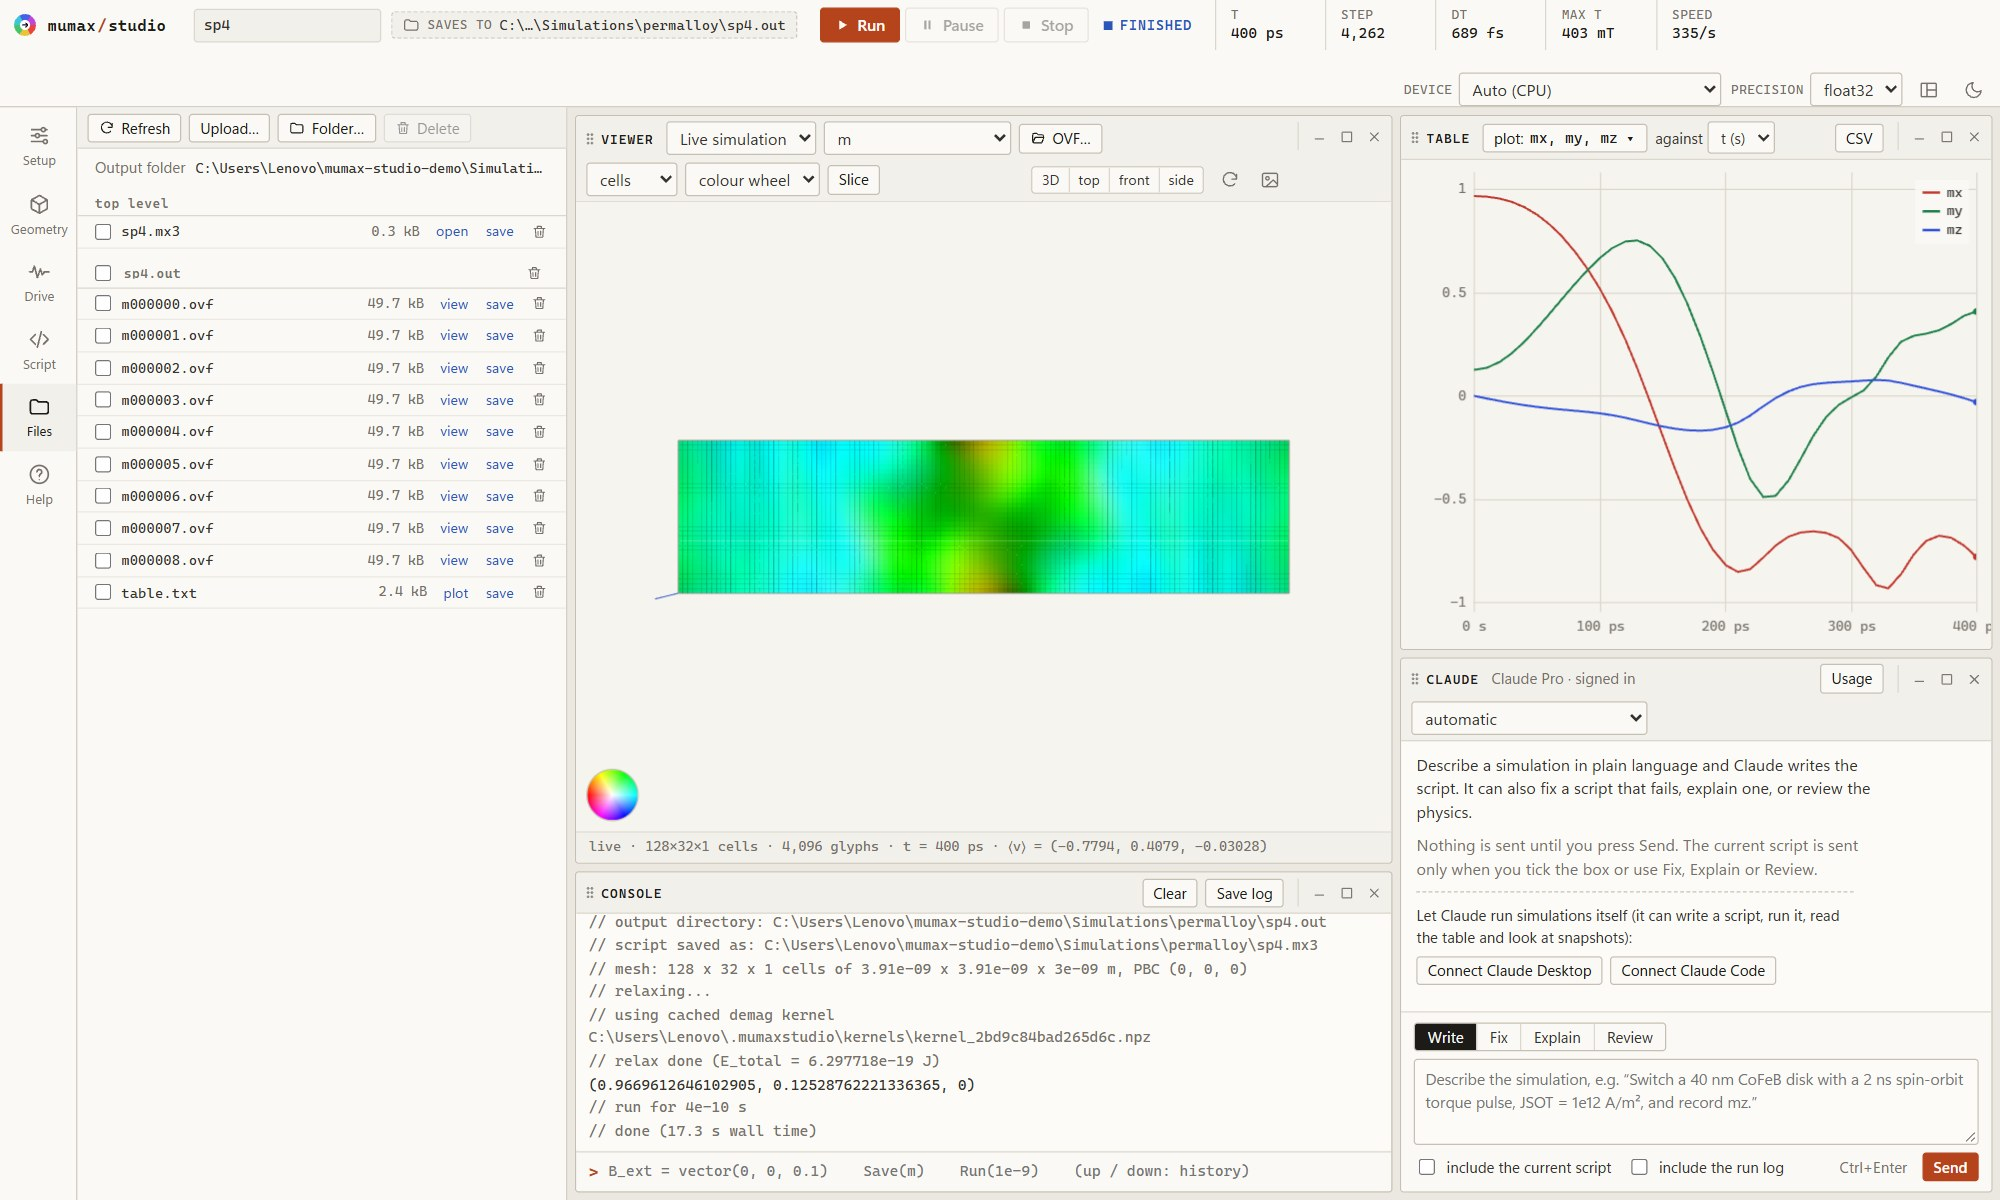
\includegraphics[width=\linewidth]{fig/ui_light.jpg}}{\fbox{\parbox[c][5cm][c]{0.9\linewidth}{\centering screenshot}}}
\caption{The main window after standard problem 4. Left: the page rail and the Files page with the output
folder. Centre: the viewer, seen from the top with the magnetization drawn as cells, and the console. Right: the
table plot and the Claude panel. The \menu{saves to} chip in the top bar shows where the run was written.}
\label{fig:ui}
\end{figure}

\section{Choosing where results are saved}\label{sec:folder}

Every run writes its results to a folder named after the simulation, \code{<name>.out}, inside the
\emph{output folder}, and keeps a copy of its script next to it as \code{<name>.mx3} or \code{<name>.py}. The
output folder can be any folder on the computer: a project folder, a shared drive, an external disk.

\paragraph{The folder must be chosen first.} No simulation runs before you have said where its results go. Until
then the chip in the top bar reads \menu{saves to: not set}, and pressing \menu{Run} opens the dialog
\menu{Where should the results be saved?} instead of starting the run. Choose a folder (the field suggests
\code{\textasciitilde/mumax-studio}) and press \menu{Use this folder}; the run then continues. Cancel, and nothing
runs. The choice is asked for once: it is remembered for the next sessions, and changed at any time with the chip.

The chip labelled \menu{saves to} in the top bar always shows the full path of the next run's result folder; hover
over it to read the path in full. Click it to open the \menu{Output folder} dialog (Figure~\ref{fig:dlgfolder}):
\begin{itemize}
\item type or paste a full path, for example \code{D:\textbackslash{}simulations\textbackslash{}thesis} or
\code{/home/me/sims}; a folder that does not exist yet is created;
\item in the desktop window, \menu{Browse\ldots} opens the system folder picker;
\item \menu{Recent} lists folders used before, and \menu{Default} returns to \code{\textasciitilde/mumax-studio};
\item \menu{Show the paths and ask before every run} switches the confirmation described below on or off.
\end{itemize}
\menu{Use this folder} checks that the folder can be written to and switches to it. The choice is remembered for
the next start, and the \menu{Files} page, uploads (STL models, mask images, waveform files) and the MCP server
used by Claude (Chapter~\ref{ch:claude}) follow it. The command-line option \code{--workspace DIR} overrides the
remembered folder for one session.

\begin{figure}[htbp]
\centering
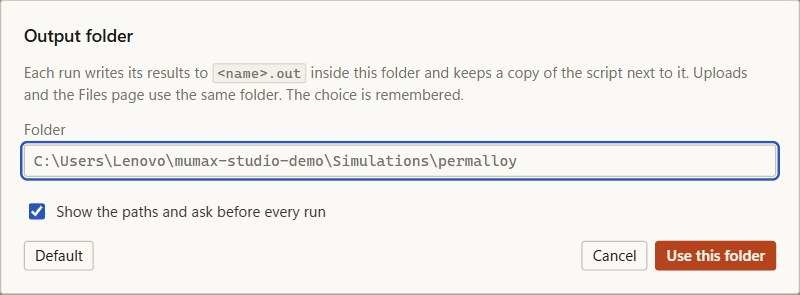
\includegraphics[width=0.78\linewidth]{fig/dlg_folder.jpg}
\caption{The \menu{Output folder} dialog, opened from the \menu{saves to} chip or from \menu{Folder\ldots} on the
Files page.}
\label{fig:dlgfolder}
\end{figure}

\paragraph{Before a run.} When \menu{Run} is pressed, a dialog states exactly where the run will write
(Figure~\ref{fig:dlgrun}): the result folder and the path of the script copy. If a result folder of the same name
already holds output files, it says how many will be replaced; rename the simulation in the top bar to keep them.
\menu{Change folder\ldots} picks another output folder without leaving the dialog. Tick \menu{Don't ask again} to
skip the dialog in future; the path remains visible in the top bar, and the first two lines of every run log in
the console repeat it:
\begin{shell}
// output directory: D:\simulations\thesis\sp4.out
// script saved as: D:\simulations\thesis\sp4.mx3
\end{shell}

\begin{figure}[htbp]
\centering
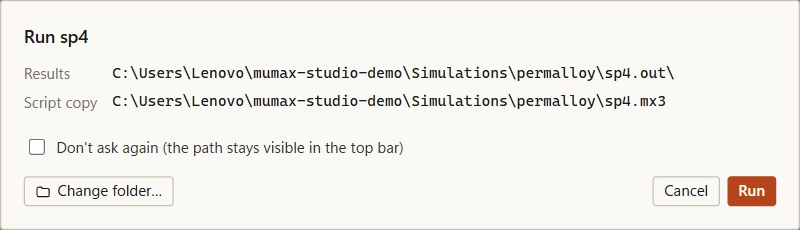
\includegraphics[width=0.78\linewidth]{fig/dlg_run.jpg}
\caption{The confirmation shown before each run, with the full paths of the results and of the script copy.}
\label{fig:dlgrun}
\end{figure}

\section{Standard problem 4}

The muMAG standard problem 4 is the usual first test of a micromagnetic code: a permalloy film of
$500\times125\times3$\,nm$^3$ is relaxed into an S state and then reversed by a field applied at an angle. Open the
\menu{Script} page and choose \menu{Examples} $\rightarrow$ \menu{01 standard problem 4}, or type:
\begin{mxcode}
SetGridSize(128, 32, 1)
SetCellSize(500e-9/128, 125e-9/32, 3e-9)

Msat  = 800e3        // A/m
Aex   = 13e-12       // J/m
alpha = 0.02

m = Uniform(1, .1, 0)
Relax()
Print(m.Average())   // S state

B_ext = vector(-24.6e-3, 4.3e-3, 0)
TableAutoSave(10e-12)
Run(1e-9)
\end{mxcode}
Set the simulation name in the top bar to \code{sp4}, press \menu{Run} or Ctrl+Enter, and confirm the paths.
The state indicator in the top bar changes from \menu{idle} to \menu{running}; the viewer shows the magnetization
in three dimensions in the mumax3 colour wheel (hue gives the in-plane direction, brightness the out-of-plane
component), refreshed about once a second, and the plot shows the columns of the table as they are written. For a
thin film the camera button \menu{top} gives the familiar flat picture; with \menu{cells} as the glyph it looks
like the field view of mumax3.

After the relaxation the console prints approximately $\langle\mathbf m\rangle = (0.9670, 0.1253, 0)$. The
mumax3 reference value of $\langle m_y\rangle$ is $0.12521$. During the reversal $\langle m_x\rangle$ crosses
zero at about $0.14$\,ns, as in the published solutions.

\section{Where the results are}

Each run writes to \code{<name>.out} in the output folder: \code{table.txt} (one row per saved time, tab
separated, with the units in the header), one OVF file for every \code{Save} or \code{AutoSave}, PNG files from
\code{Snapshot} and figures from Python scripts. The \menu{Files} page lists the output folder
(Section~\ref{sec:files}): \menu{view} shows an OVF file in the viewer, \menu{plot} draws a table, \menu{open}
loads a script into the editor, \menu{save} writes a copy anywhere you choose, and the bin button deletes.

\paragraph{Saving the script.} The script is copied next to its results at every run. To keep it somewhere else,
press \menu{Save\ldots} on the \menu{Script} page. The dialog (Figure~\ref{fig:dlgsave}) shows the full path it
will write, by default \code{<output folder>/<name>.mx3}. Edit the path to save anywhere, use \menu{Browse\ldots} in
the desktop window, or give a bare file name to save in the output folder. An existing file is replaced only after
a confirmation. \menu{Download copy} hands the file to the browser instead.

\begin{figure}[htbp]
\centering
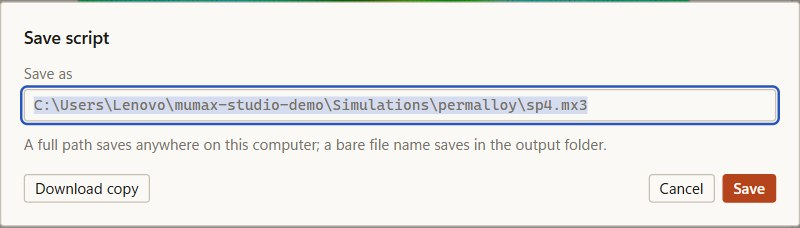
\includegraphics[width=0.78\linewidth]{fig/dlg_save.jpg}
\caption{\menu{Save script}: the full path is shown, and can be changed, before anything is written.}
\label{fig:dlgsave}
\end{figure}

\section{Changing parameters during a run}

The console accepts any statement of the script language while a simulation runs. It is executed between two
solver steps:
\begin{mxcode}
alpha = 0.5
B_ext = vector(0, 0, 0.1)
\end{mxcode}
\menu{Pause} stops the solver without losing the state; \menu{Stop} ends the run.

% =====================================================================
\chapter{The window and its panels}\label{ch:ui}

\section{Pages}

\begin{center}
\begin{tabular}{>{\bfseries}l p{0.72\linewidth}}
\toprule
Setup & Material presets (permalloy, CoFeB, Co/Pt with DMI, YIG and others), per-region values, initial state,
solver, temperature and the table columns. \\
Geometry & Mesh, then a stack of shapes combined by union, difference, intersection and exclusive or. \\
Drive & Applied field \code{B\_ext}, spin-transfer current \code{J} and spin-orbit current \code{JSOT}, each a sum of
terms. \\
Script & The script that the forms generate. Once edited by hand it no longer follows the forms.
\menu{Save\ldots} writes it to a path you choose. \\
Files & The output folder: results of each run, uploads (STL, PNG and CSV files used by shapes and waveforms);
viewing, plotting, copying and deleting files. \\
Help & A summary of the script language, the mumax+ interface, the viewer and the assistant. \\
\bottomrule
\end{tabular}
\end{center}

\section{Arranging the panels}

The right-hand side of the window is a dock: a tree of horizontal and vertical splits whose leaves are panels.
Every panel has a title bar with three buttons, \menu{minimise}, \menu{maximise} and \menu{close}.
\begin{itemize}
\item Drag a divider to change the share of two neighbours. Double-click a divider to make them equal; with a
divider focused, the arrow keys move it.
\item Drag a panel by its title onto another panel. Dropping on an edge places it beside that panel; dropping in
the centre exchanges the two.
\item Minimise reduces a panel to its title bar, or to a narrow strip in a horizontal split. Maximise lets one
panel fill the dock; Escape restores the layout.
\item The \menu{Panels} menu reopens closed panels and offers four arrangements: \menu{Standard},
\menu{Large viewer}, \menu{Analysis} (viewer and plot side by side) and \menu{Writing with Claude}.
\end{itemize}
The layout is saved on the computer and restored at the next start, together with the chosen device, precision
and colour theme. Figure~\ref{fig:dark} shows the dark colour theme, selected with the moon button at the right of the
top bar.

\begin{figure}[htbp]
\centering
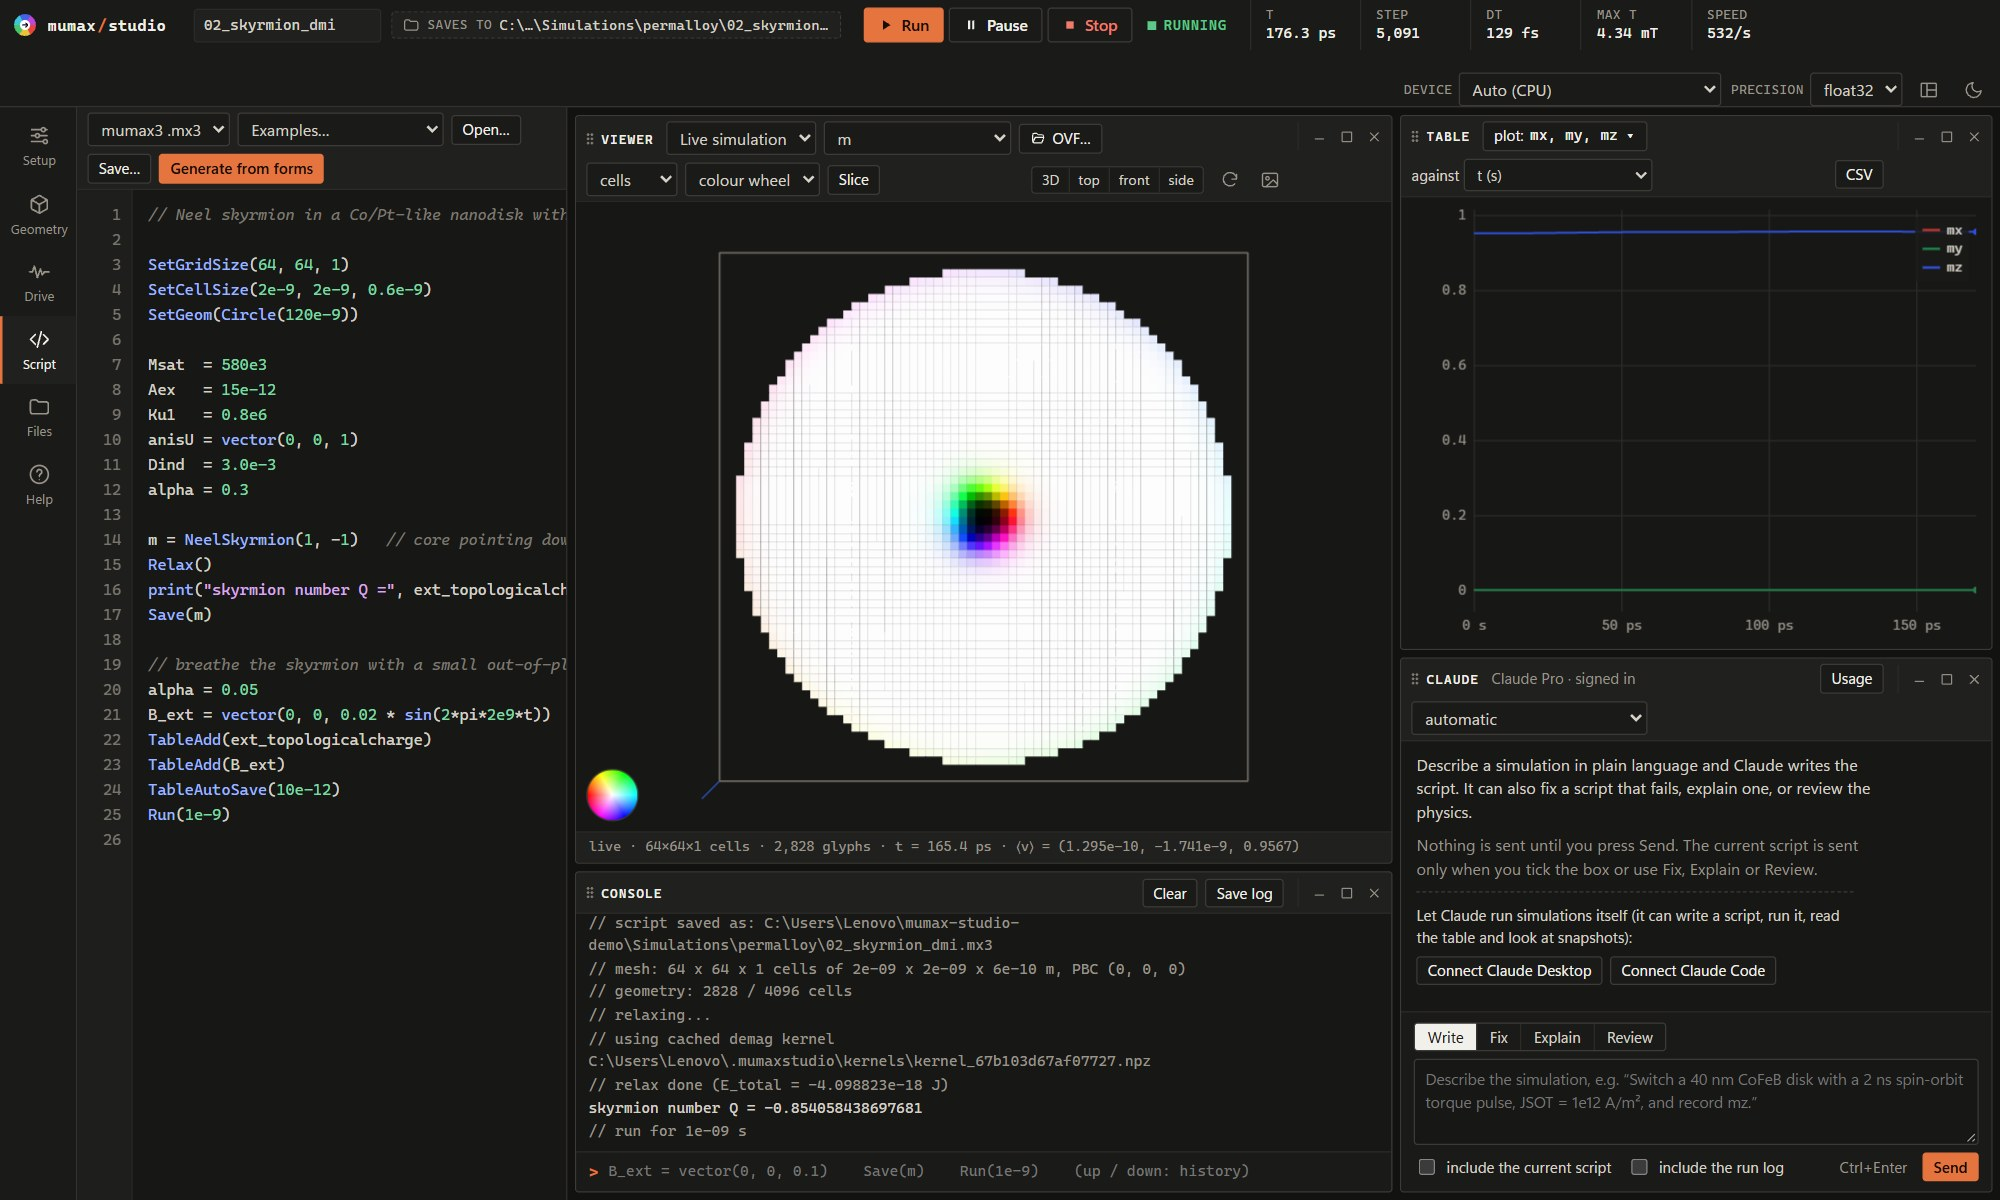
\includegraphics[width=\linewidth]{fig/ui_dark.jpg}
\caption{The dark colour theme, with the skyrmion example running and the viewer seen from the top.}
\label{fig:dark}
\end{figure}

\section{Device and precision}

The \menu{Device} menu in the top bar lists \menu{Auto}, \menu{CPU} and every GPU found, each with its name.
A GPU that failed its self-test is shown but disabled, with the reason beside it. The choice applies to the next
run; the line under the menu states which device the next run will use, or which device the current run is using.
\menu{Precision} selects single (float32) or double (float64) arithmetic. Single precision is the mumax3 default and
is about twice as fast; double precision is advisable for energy minimisation of large, nearly uniform states and
for very small time steps.

% =====================================================================
\chapter{The mumax3 script language}\label{ch:mx3}

The language is that of mumax3: a small subset of Go with case-insensitive names. This chapter describes the
parts that are used in nearly every simulation; the Help page lists all functions.

\section{Mesh}
\begin{mxcode}
SetGridSize(Nx, Ny, Nz)      // number of cells
SetCellSize(cx, cy, cz)      // metres
SetPBC(Px, Py, Pz)           // periodic images in each direction, 0 = open
\end{mxcode}
Choose the cell size below the exchange length $l_\text{ex} = \sqrt{2A/(\mu_0 M_s^2)}$ (about 5\,nm for
permalloy). Powers of two, or products of small primes, make the FFT fastest.

\section{Material parameters}

Parameters are assigned globally or per region:
\begin{mxcode}
Msat = 800e3
Aex  = 13e-12
Ku1  = 0.5e6;  anisU = vector(0, 0, 1)
Dind = 1.5e-3                     // interfacial DMI, J/m^2
DefRegion(1, Circle(50e-9))
Msat.SetRegion(1, 1.1e6)
ext_ScaleExchange(0, 1, 0.5)      // exchange between regions 0 and 1
\end{mxcode}
Any parameter can depend on time through the variable \code{t}; the expression is re-evaluated at every step:
\begin{mxcode}
B_ext = vector(0, 0, 0.01*sin(2*pi*1e9*t))
\end{mxcode}

\section{Initial states}

\code{Uniform}, \code{Vortex(circ, pol)}, \code{NeelSkyrmion(charge, pol)}, \code{BlochSkyrmion},
\code{TwoDomain}, \code{RandomMag} and \code{RandomMagSeed} create states; \code{.Transl}, \code{.Scale} and
\code{.Add} move and combine them. A previous result is loaded with \code{m.LoadFile("m000010.ovf")}.

\section{Running}
\begin{center}
\begin{tabular}{>{\ttfamily}l p{0.66\linewidth}}
\toprule
Run(T) & integrate the LLG equation for a time $T$ \\
Steps(n) & take $n$ solver steps \\
RunWhile(cond) & run while a condition holds, e.g.\ \code{RunWhile(m.comp(2).average() > 0)} \\
Relax() & remove precession and lower the energy until the torque stops decreasing \\
Minimize() & steepest-descent energy minimisation (faster than \code{Relax} for static states) \\
SetSolver(k) & 1 Euler, 2 Heun, 3 Bogacki--Shampine, 4 RK4, 5 Dormand--Prince (the default); 6 (Fehlberg) is
mapped to 5 and $-1$ (backward Euler) to Heun \\
\bottomrule
\end{tabular}
\end{center}
\code{MaxErr}, \code{MinDt}, \code{MaxDt} and \code{FixDt} control the time step as in mumax3.

\section{Output}
\begin{mxcode}
TableAdd(E_total)           // add a column
TableAutoSave(10e-12)       // one row every 10 ps
AutoSave(m, 50e-12)         // an OVF file every 50 ps
Save(B_demag)               // once, now
SaveAs(m, "relaxed")
Snapshot(m)                 // PNG image
\end{mxcode}
Any quantity can be read at a single cell with \code{GetCell}: \code{m.GetCell(10, 5, 0)} returns the vector in
cell $(10, 5, 0)$, and \code{Msat.GetRegion(1)} the value of a parameter in a region.

\section{Control flow}

Loops, conditions and functions follow Go:
\begin{mxcode}
for B := 0.0; B <= 0.1; B += 0.01 {
    B_ext = vector(B, 0, 0)
    Minimize()
    TableSave()
}
\end{mxcode}

% =====================================================================
\chapter{Geometry and regions}\label{ch:geometry}

The geometry says which cells of the mesh are magnetic; regions label cells so that material parameters,
fields and currents can differ from one part of the magnet to another. There are three ways to build a
geometry, and they produce the same thing in the end, a script:
\begin{itemize}
\item the \menu{Geometry} page, where shapes are added, combined and moved with the mouse
(Section~\ref{sec:geomui});
\item shape expressions in a script, \code{.mx3} or Python (Section~\ref{sec:geommx3});
\item Python code that computes the geometry: loops, NumPy, random numbers, arrays (Section~\ref{sec:geompy}).
\end{itemize}

\section{Coordinates}

All three use the conventions of mumax3. The mesh is a box of $N_x\times N_y\times N_z$ cells of size
$c_x\times c_y\times c_z$, centred on the origin: $x$ runs from $-N_xc_x/2$ to $+N_xc_x/2$, and so on. A cell
belongs to a shape when its \emph{centre} lies inside it. Lengths are in metres in scripts and in nanometres in
the forms of the Geometry page. A shape larger than the box is simply cut off at the box; a cell outside every
shape is empty (\code{Msat} is zero there). With \code{EdgeSmooth = n} (\menu{edge smooth} on the Geometry page)
each edge cell is sampled at $n^3$ points and given a partial volume, which reduces the staircase error of curved
edges, as in mumax3.

\section{Building a geometry in the interface}\label{sec:geomui}

\subsection{The Geometry page}

The page has two parts. \menu{Mesh} sets $N_x$, $N_y$, $N_z$, the periodic repetitions (\menu{PBC}, for example
\code{0,0,0} or \code{4,4,0}), the cell size in nanometres and \menu{edge smooth}. The line beneath gives the size
of the box, the number of cells and the exchange length of the material on the Setup page, and warns when the
cells are larger than the exchange length.

\menu{Shapes} is an ordered list. The first shape defines the magnet, each further shape modifies it with its
\emph{operation}:
\begin{center}
\begin{tabular}{>{\bfseries}l l p{0.55\linewidth}}
\toprule
Badge & Operation & Effect \\
\midrule
$\cup$ & add to magnet & union: cells inside the shape become magnetic \\
$-$ & cut out & difference: cells inside the shape become empty \\
$\cap$ & intersect & only cells inside both the magnet so far and the shape remain \\
$\oplus$ & toggle (xor) & cells inside exactly one of the two remain \\
R & region only & the magnet is not changed; the shape only assigns its region number \\
\bottomrule
\end{tabular}
\end{center}
Because the operations are applied from the top of the list down, the order matters: a hole cut out and then
covered by a later \menu{add} is filled again. The arrow buttons on each entry move it up or down, the eye button
hides it without deleting it, the copy button duplicates it (Shift+D) and the cross removes it (Delete).

Selecting an entry opens its editor below the list: a name, the operation, the dimensions of the shape in
nanometres, a \menu{Transform} (position $x, y, z$; rotation about $z$, $x$ and $y$ in degrees; a scale factor;
\menu{repeat every x / y} for periodic arrays) and \menu{region (0 = none)}.

The available shapes are, in the \menu{Add shape\ldots} menu:
\begin{description}
\item[2D, extruded through the film:] Rectangle, Disk, Ellipse, Ring, Regular polygon, Polygon (vertices typed as
\code{x,y; x,y; \ldots} in nanometres).
\item[3D:] Cuboid, Cylinder, Ellipsoid, Sphere, Cone, Torus, and Layers, which selects a range of layer indices
$z_0 \le i_z < z_1$ over the whole $xy$ plane (useful for multilayers).
\item[Imported:] a 3D model from an STL file (exported from Blender, FreeCAD, OpenSCAD, \ldots) and an image mask
(PNG or JPG; dark, opaque pixels are magnetic, and the image is stretched over the $xy$ extent of the box).
\item[Code:] \menu{Custom inside(x, y, z)}, a Python expression in the cell-centre coordinates; see
Section~\ref{sec:geompy}.
\end{description}
For STL models and images the editor has an \menu{Upload\ldots} button that copies the file into the output
folder, where the script finds it. An STL file needs the size of its unit (\menu{nm per file unit}: 1 for a model
drawn in nanometres, 1000 for micrometres) and a voxel resolution along its longest side; the model is centred on
the origin before the transform is applied.

\subsection{The preview}

While the Geometry page is open, the viewer shows the geometry rather than a field (Figure~\ref{fig:geom2d}). Two
buttons in its title bar choose the view:
\begin{description}
\item[2D edit] shows one layer from above; the slider \menu{z} chooses the layer. Magnetic cells are drawn in
the colour of their region, the selected shape is outlined, and a cross marks its origin. Here shapes are edited
with the mouse: drag to move the selected shape (it snaps to half cells; hold Alt to move freely), Shift and the
wheel to rotate, Ctrl and the wheel to scale, the arrow keys to move by one cell (ten with Shift), \code{R} to
rotate by $15^\circ$. Clicking a shape selects it.
\item[3D] shows the whole magnet as cells coloured by region (Figure~\ref{fig:geom3d}): grey for region~0 and
one colour per region number. Orbit, pan and zoom as for fields (Chapter~\ref{ch:output}); \menu{Slice} cuts the body open to look
inside.
\end{description}
The preview is computed by the engine itself, with the same code that the run uses, so what is shown is what will
be simulated, including STL models, images and custom code. The info line gives the number of magnetic cells, the
same number that the run prints as \code{// geometry: N / M cells}.

\begin{figure}[htbp]
\centering
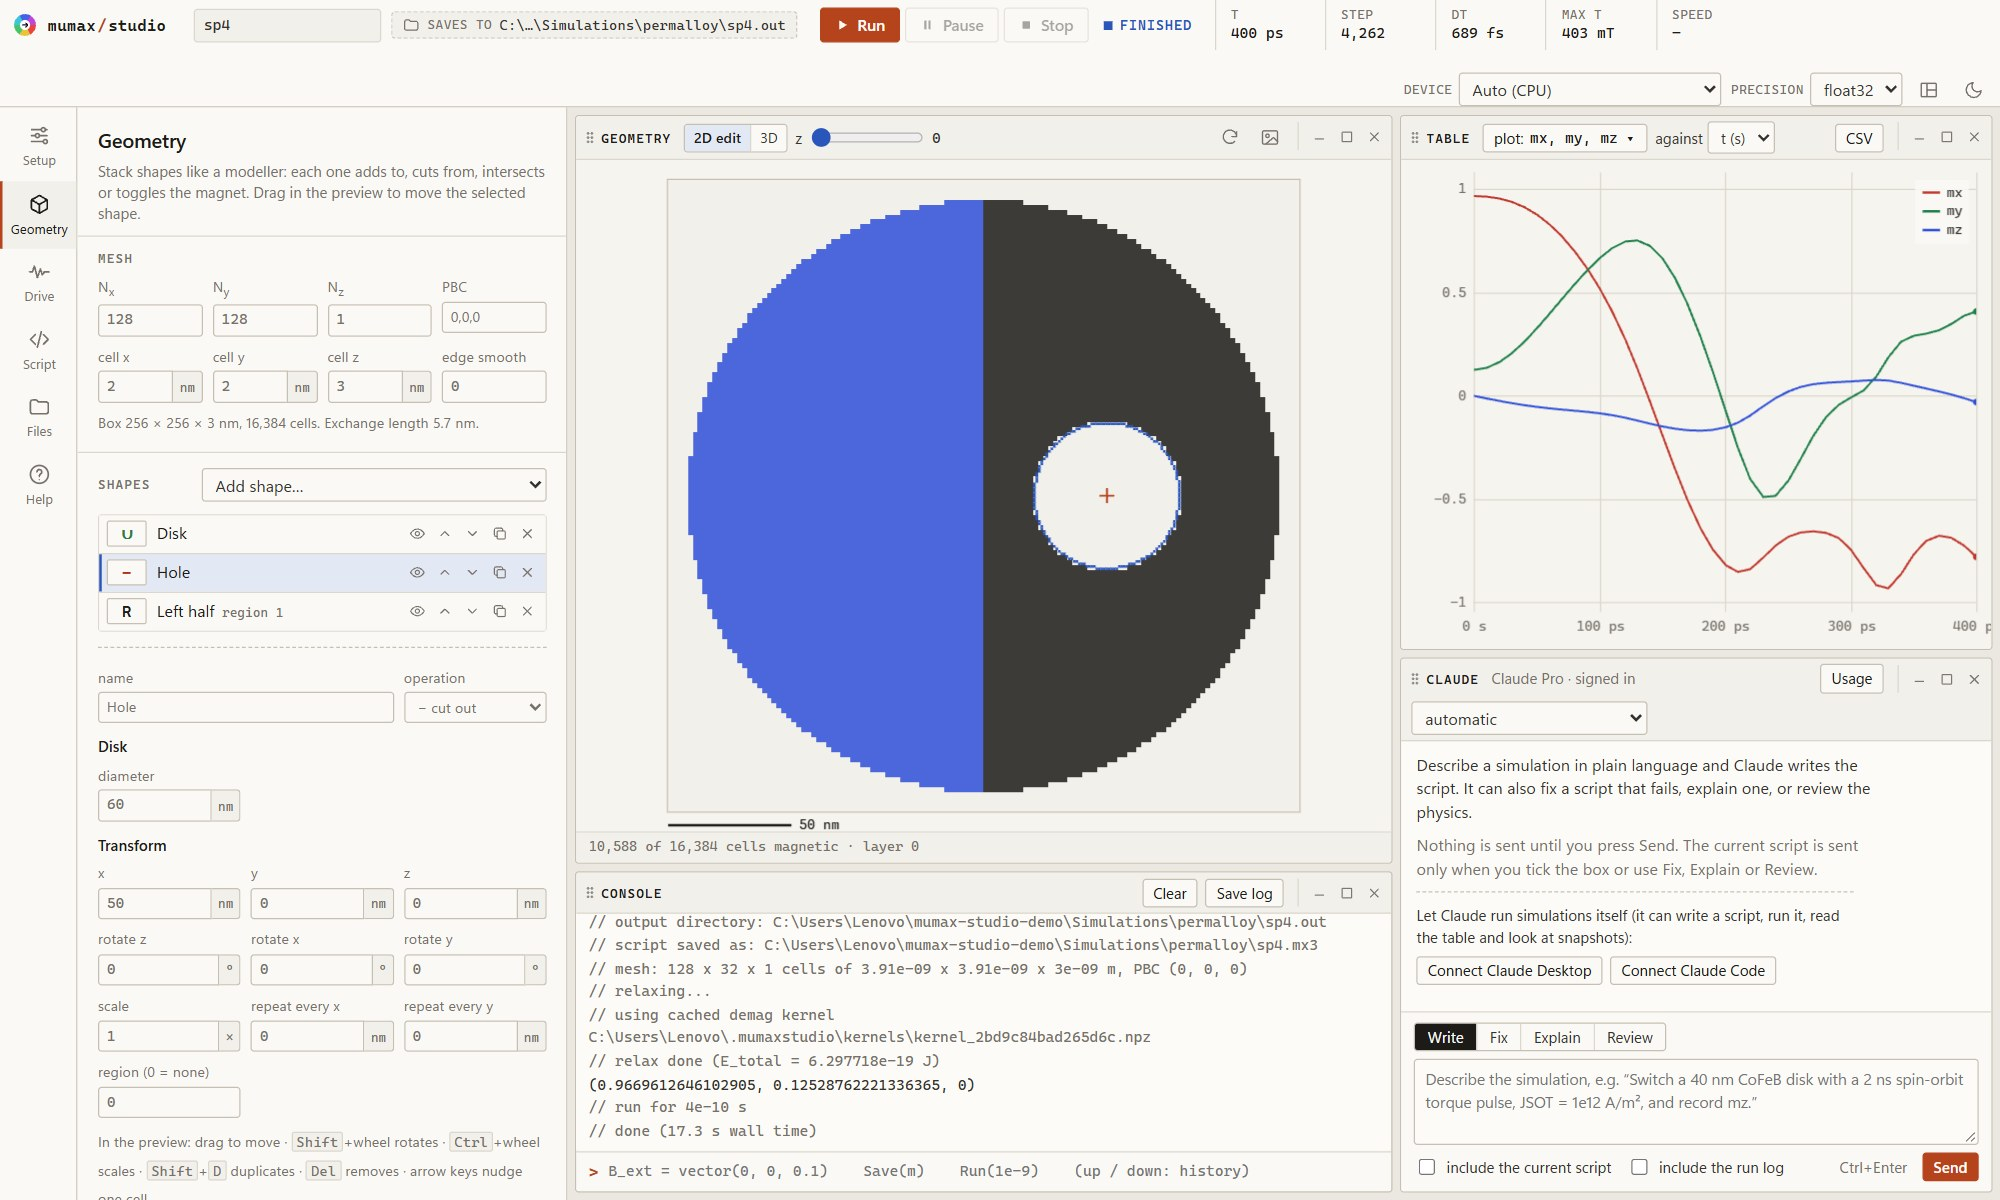
\includegraphics[width=\linewidth]{fig/geom_2d.jpg}
\caption{The Geometry page building a disk with an off-centre hole. The list holds a disk ($\cup$), a smaller
disk cut out of it ($-$, selected, outlined in the preview) and a rectangle that only assigns region~1 to the
left half (R). The viewer is in \menu{2D edit} mode.}
\label{fig:geom2d}
\end{figure}

\begin{figure}[htbp]
\centering
\begin{minipage}{0.49\linewidth}\centering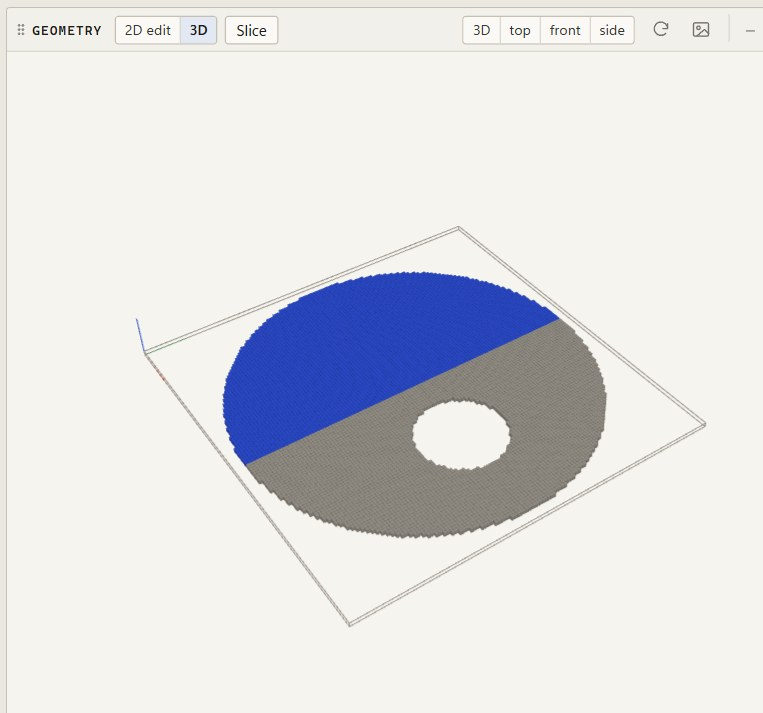
\includegraphics[width=\linewidth]{fig/geom_3d.jpg}\end{minipage}\hfill
\begin{minipage}{0.49\linewidth}\centering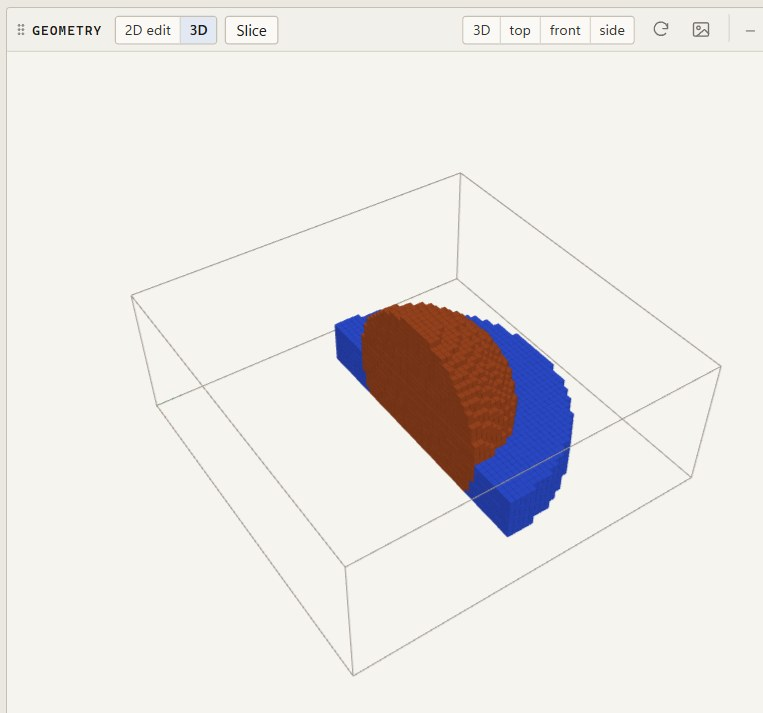
\includegraphics[width=\linewidth]{fig/geom_3d_stack.jpg}\end{minipage}
\caption{The \menu{3D} geometry view. Left: the disk with a hole of Figure~\ref{fig:geom2d}, region~1 in blue.
Right: a three-dimensional body on a $64\times64\times24$ mesh: a cylinder (region~1, blue) with a sphere on top
(region~2), the front half cut away by a cuboid with the operation \menu{cut out}.}
\label{fig:geom3d}
\end{figure}

\subsection{Example: a disk with an off-centre hole}

\begin{enumerate}
\item On the Geometry page set the mesh to $N_x = N_y = 128$, $N_z = 1$, cells of $2\times2\times3$\,nm$^3$.
\item \menu{Add shape\ldots} $\rightarrow$ \menu{Disk}; set its diameter to 240\,nm.
\item \menu{Add shape\ldots} $\rightarrow$ \menu{Disk} again; set the operation to \menu{cut out}, the diameter
to 60\,nm, and $x$ to 50\,nm, or drag it to the right in the preview.
\item To give the left half other material values, add a \menu{Rectangle} of $128\times256$\,nm$^2$ at
$x = -64$\,nm, set its operation to \menu{region only} and its region to 1. On the Setup page open
\menu{Per-region values}, \menu{Add value}, and choose for example region 1, \code{Msat}, 600\,kA/m.
\item Press \menu{3D} in the viewer to check the result, then \menu{Generate from forms} on the Script page.
\end{enumerate}
The generated script contains the geometry as ordinary script code, which can be edited further:
\begin{mxcode}
SetGridSize(128, 128, 1)
SetCellSize(2e-9, 2e-9, 3e-9)

// geometry
magnet := Circle(2.4e-7)
magnet = magnet.Sub(Circle(6e-8).Transl(5e-8, 0, 0))
SetGeom(magnet)
DefRegion(1, Rect(1.28e-7, 2.56e-7).Transl(-6.4e-8, 0, 0))
...
Msat.SetRegion(1, 6e5)
\end{mxcode}
The magnet has 10\,588 of the 16\,384 cells.

\subsection{Example: a nanowire with a notch and a pinning region}

A domain-wall track: a $2048\times100$\,nm$^2$ wire on a $512\times32\times1$ mesh of $4\times4\times2$\,nm$^3$
cells. Add a \menu{Rectangle} of $2048\times100$\,nm$^2$; add a second \menu{Rectangle} of $40\times60$\,nm$^2$
with \menu{cut out} at $y = 30$\,nm, which makes a notch in the upper edge at the centre. Then add a
\menu{Rectangle} of $150\times100$\,nm$^2$ at $x = -950$\,nm with \menu{region only}, region~1, and on the Setup
page give region~1 a higher anisotropy, for example \code{Ku1} = 1\,MJ/m$^3$, to hold the wall at the start of the
track. The equivalent script is
\begin{mxcode}
SetGridSize(512, 32, 1)
SetCellSize(4e-9, 4e-9, 2e-9)
wire := Rect(2048e-9, 100e-9)
notch := Rect(40e-9, 60e-9).Transl(0, 30e-9, 0)
SetGeom(wire.Sub(notch))
DefRegion(1, XRange(-inf, -900e-9))
\end{mxcode}

\subsection{Example: a periodic array}

The \menu{repeat every x} and \menu{repeat every y} fields turn one shape into an infinite lattice with that
period, cut off by the box. A disk of 100\,nm with \menu{repeat every x} = \menu{repeat every y} = 150\,nm gives a
square lattice of dots; with the operation \menu{cut out} on top of a rectangle it gives an antidot lattice. In
scripts this is \code{Circle(100e-9).Repeat(150e-9, 150e-9, 0)}. Combine it with \menu{PBC} to simulate an
extended lattice from one unit cell.

\subsection{Example: layers and three-dimensional bodies}

For a stack of films, set $N_z$ to the number of layers and use \menu{Layers} entries with \menu{region only} to
label them: layers $0$--$1$ region~1, layer $1$--$2$ region~2 (a spacer) and so on. Three-dimensional bodies are
built from the 3D shapes: the right-hand picture of Figure~\ref{fig:geom3d} is a \menu{Cylinder} of 150\,nm
diameter and 24\,nm height at $z = -24$\,nm (region~1), a \menu{Sphere} of 96\,nm at $z = -12$\,nm (region~2) and a
\menu{Cuboid} of $200\times100\times100$\,nm$^3$ at $y = -50$\,nm with \menu{cut out}, on a mesh of
$64\times64\times24$ cells of 3\,nm. Use the \menu{3D} view and its \menu{Slice} menu to look inside.

\section{Geometry in scripts}\label{sec:geommx3}

\code{SetGeom(shape)} restricts the magnet to a shape and \code{DefRegion(n, shape)} assigns region $n$
($0\le n\le255$) to the cells inside a shape; a later \code{DefRegion} overwrites an earlier one where they
overlap. The shapes are
\begin{center}
\small
\begin{tabular}{>{\ttfamily\raggedright}p{0.42\linewidth} p{0.5\linewidth}}
\toprule
Circle(d), Ellipse(dx, dy), Rect(w, h), Square(a) & 2D, through the whole thickness \\
Ring(dout, din), RegularPolygon(n, d), Polygon(xs, ys) & 2D additions of mumax Studio \\
Cylinder(d, h), Cuboid(a, b, c), Ellipsoid(dx, dy, dz), Cone(d, h), Sphere(d), Torus(D, d) & 3D \\
XRange(a, b), YRange(a, b), ZRange(a, b) & half-spaces and slabs \\
Layers(i0, i1), Layer(i), Cell(ix, iy, iz) & by cell index \\
Universe() & the whole box \\
ImageShape("mask.png") & dark pixels of an image \\
STLShape("part.stl", 1e-9) & a triangle mesh, here in nanometres \\
\bottomrule
\end{tabular}
\end{center}
Every shape has the transforms \code{Transl(x, y, z)}, \code{RotX/RotY/RotZ(angle)} (radians),
\code{Scale(sx, sy, sz)} and \code{Repeat(px, py, pz)}, and the combinations \code{Add}, \code{Sub},
\code{Intersect}, \code{Xor} and \code{Inverse}. Each returns a new shape, so they chain:
\begin{mxcode}
SetGeom(Circle(240e-9).Sub(Circle(60e-9).Transl(50e-9, 0, 0)))    // disk with a hole
SetGeom(RegularPolygon(3, 200e-9).RotZ(pi/2))                      // triangle
SetGeom(Cylinder(150e-9, 60e-9).Add(Sphere(80e-9).Transl(0, 0, 40e-9)))
SetGeom(STLShape("part.stl", 1e-9).RotZ(pi/4))
EdgeSmooth = 8
\end{mxcode}
Grains are made with \code{ext\_makegrains(size, nregions, seed)}, a Voronoi tessellation of the film into
regions $0\ldots n-1$, whose parameters can then be varied region by region.

\section{Generating geometry with Python}\label{sec:geompy}

In a Python script (\code{.py}, Chapter~\ref{ch:python}) all the shapes above are available, and the full language
can be used to produce them. Python can generate geometry in four ways.

\paragraph{1. A function of position.} \code{SetGeom} and \code{DefRegion} accept any function
\code{inside(x, y, z)} that returns \code{True} for magnetic cells. It is called once with NumPy arrays of the
cell-centre coordinates in metres (broadcastable arrays of shapes $(1,1,N_x)$, $(1,N_y,1)$ and $(N_z,1,1)$), so
it must use NumPy operations: \code{\&}, \code{|} and \code{\textasciitilde} rather than \code{and}, \code{or} and
\code{not}.
\begin{pycode}
SetGridSize(128, 128, 1); SetCellSize(2e-9, 2e-9, 3e-9)
r2 = lambda x, y: x**2 + y**2
SetGeom(lambda x, y, z: (r2(x, y) < (120e-9)**2) & (r2(x, y) > (40e-9)**2))   # annulus
DefRegion(1, lambda x, y, z: x > 0)                                          # right half
\end{pycode}
A function that only accepts single numbers also works (it is then evaluated cell by cell, which is slower).
\code{Shape(f)} turns a function into a shape object, so that it can be combined and transformed like the others:
\code{Shape(f).Sub(Circle(50e-9)).RotZ(0.3)}.

\paragraph{2. Shapes built in a loop.} Shape objects can be accumulated in ordinary Python loops. An antidot
lattice of $9\times5$ holes:
\begin{pycode}
SetGridSize(256, 128, 1); SetCellSize(4e-9, 4e-9, 4e-9)
film = Rect(1000e-9, 500e-9)
for ix in range(-4, 5):
    for iy in range(-2, 3):
        film = film.Sub(Circle(40e-9).Transl(ix*110e-9, iy*110e-9, 0))
SetGeom(film)
\end{pycode}
The same pattern assigns a region to every element of an array, here four rings in a row:
\begin{pycode}
SetGridSize(256, 64, 1); SetCellSize(4e-9, 4e-9, 4e-9)
rings = [Ring(200e-9, 120e-9).Transl((k - 1.5)*250e-9, 0, 0) for k in range(4)]
magnet = rings[0]
for r in rings[1:]:
    magnet = magnet.Add(r)
SetGeom(magnet)
for k, r in enumerate(rings):
    DefRegion(k + 1, r)          # regions 1..4, one per ring
\end{pycode}

\paragraph{3. Random geometry with NumPy.} Random defects, grains or rough edges come from NumPy's random
generator; a fixed seed makes the geometry reproducible:
\begin{pycode}
import numpy as np
SetGridSize(128, 128, 1); SetCellSize(4e-9, 4e-9, 4e-9)
rng = np.random.default_rng(7)
centres = rng.uniform(-230e-9, 230e-9, size=(25, 2))
def inside(x, y, z):
    keep = np.ones(np.broadcast(x, y).shape, dtype=bool)
    for cx, cy in centres:
        keep &= (x - cx)**2 + (y - cy)**2 > (15e-9)**2
    return keep
SetGeom(inside)               # a film with 25 random holes of 30 nm
\end{pycode}

\paragraph{4. From an array.} A geometry computed elsewhere, or read from a file (\code{np.load},
\code{np.loadtxt}, an image through Pillow), is a boolean array of the size of the mesh. Convert the
coordinates back to cell indices and look the array up:
\begin{pycode}
import numpy as np
Nx, Ny, Nz = 64, 32, 1
SetGridSize(Nx, Ny, Nz); SetCellSize(5e-9, 5e-9, 5e-9)
mask = np.zeros((Ny, Nx), dtype=bool)          # rows are y, columns are x
mask[8:24, 4:60] = True                        # a bar
mask[12:20, 28:36] = False                     # with a square hole
def from_array(x, y, z):
    ix = np.clip(np.round(x / 5e-9 + (Nx - 1) / 2).astype(int), 0, Nx - 1)
    iy = np.clip(np.round(y / 5e-9 + (Ny - 1) / 2).astype(int), 0, Ny - 1)
    return mask[iy, ix]
SetGeom(from_array)
\end{pycode}
For a three-dimensional array of shape $(N_z, N_y, N_x)$ compute \code{iz} the same way and return
\code{mask[iz, iy, ix]}. A small number of single cells can also be set with \code{DefRegionCell(n, ix, iy, iz)}.

\paragraph{Layers and multilayers.} \code{Layer(i)} and \code{Layers(i0, i1)} select by layer index, which with a
loop labels a stack; a nonmagnetic spacer is a region with \code{Msat} zero, and \code{ext\_ScaleExchange} couples
the layers across it:
\begin{pycode}
SetGridSize(64, 64, 3); SetCellSize(4e-9, 4e-9, 1e-9)
SetGeom(Circle(240e-9))
for i in range(3):
    DefRegion(i + 1, Layer(i))
Msat = 1.1e6; Aex = 15e-12
Msat.SetRegion(2, 0)                 # the middle layer is the spacer
ext_ScaleExchange(1, 3, -0.1)        # antiferromagnetic coupling across it
\end{pycode}

\paragraph{Python in the interface.} Python geometry can be used in three places in the program. On the Geometry
page, the shape \menu{Custom inside(x, y, z)} takes a Python expression, for example
\code{(x/120e-9)**2 + (y/60e-9)**2 < 1 + 0.3*np.cos(6*np.arctan2(y, x))}, a flower-shaped dot; it can be combined
with the other shapes, and the preview shows it. Using it switches the generated script to Python. On the Script
page, choose \menu{Python .py} as the language and write any of the code of this section. While a simulation runs,
geometry statements can also be typed into the console. The example \menu{12 geometry python} (Script page,
\menu{Examples}) combines the first three methods: an antidot lattice made in a loop, eight random defects and two
regions defined by a function, followed by an energy minimisation in a field.

\section{Checking a geometry}

Before a long run, look at the geometry in the \menu{3D} view of the Geometry page, and read the line
\code{// geometry: N / M cells} at the start of the run log: an empty or nearly full box usually means a unit
error (nanometres given where metres are expected). \code{Save(geom)} and \code{Save(regions)} write the
geometry and the region map as OVF files, which the viewer shows like any other field.

% =====================================================================
\chapter{Spin-transfer and spin-orbit torques}\label{ch:torques}

\section{Zhang--Li and Slonczewski torques}

The spin-transfer torque of an in-plane current uses \code{J} (A/m$^2$), the polarisation \code{Pol} and the
non-adiabaticity \code{xi}. For a perpendicular current through a fixed layer the Slonczewski form applies, with
\code{FixedLayer}, \code{Lambda}, \code{EpsilonPrime} and \code{FreeLayerThickness}. Both follow mumax3.

\section{Spin-orbit torque}

The spin-orbit torque of the STT--SOT fork is
\begin{equation}
\boldsymbol\tau_\text{SOT} = \frac{\gamma}{1+\alpha^2}\Big[(\beta+\alpha\beta_\text{FL})\,
 \mathbf m\times(\boldsymbol\sigma\times\mathbf m) + (\beta_\text{FL}-\alpha\beta)\,\boldsymbol\sigma\times\mathbf m\Big],
\end{equation}
where
\begin{equation}
\beta = \frac{\hbar\,\theta_\text{SH}\,J}{2e\,M_s\,d},\qquad \beta_\text{FL} = \beta\cdot\text{HFLoverHDL},
\end{equation}
with the parameters
\begin{center}
\begin{tabular}{>{\ttfamily}l p{0.7\linewidth}}
\toprule
JSOT & current density $J$ in the heavy metal (A/m$^2$); the $z$ component is used \\
SPINHALL & spin Hall angle $\theta_\text{SH}$ \\
HFLoverHDL & ratio of field-like to damping-like torque \\
SOThickness & free-layer thickness $d$ (m); 0 means the mesh thickness \\
SOTFixedLayer & spin polarisation direction $\boldsymbol\sigma$ \\
DisableSOTorque & switch the term off \\
\bottomrule
\end{tabular}
\end{center}

\section{Example: switching a perpendicular magnet}

\begin{mxcode}
SetGridSize(32, 32, 1)
SetCellSize(2.5e-9, 2.5e-9, 1e-9)
SetGeom(Circle(80e-9))
Msat = 1.1e6;  Aex = 15e-12;  alpha = 0.05
Ku1 = 0.9e6;   anisU = vector(0, 0, 1)
m = Uniform(0, 0, 1)

SPINHALL      = 0.3
HFLoverHDL    = 0.2
SOTFixedLayer = vector(0, 1, 0)
B_ext = vector(0.02, 0, 0)                     // symmetry-breaking in-plane field
JSOT  = vector(0, 0, 3e12*Trapezoid(t, 0.1e-9, 50e-12, 1e-9, 50e-12))

TableAutoSave(5e-12)
Run(3e-9)
\end{mxcode}
The anisotropy field of this film is $2K_{u1}/M_s - \mu_0 M_s \approx 0.25$\,T and the damping-like amplitude
is $\beta \approx 0.27$\,T, so the current is above the switching threshold. During the 1\,ns pulse the
magnetization is held close to the plane ($\langle m_z\rangle \approx 0.1$); after the pulse it falls into the
lower energy minimum, with $\langle m_z\rangle = -0.85$ at 3\,ns and still precessing. With \code{JSOT} of the
opposite sign the same pulse returns it to the upper state ($\langle m_z\rangle = +0.85$ at 3\,ns). At half the
current, $1.5\times10^{12}$\,A/m$^2$, the magnet does not switch: $\langle m_z\rangle$ only dips to $0.8$.

\section{Pulse shapes and spatial profiles}

The drive library provides waveforms of unit height that can be multiplied into any expression:
\code{Pulse}, \code{Step}, \code{Ramp}, \code{SmoothStep}, \code{Gaussian(t, t0, fwhm)},
\code{Trapezoid(t, t0, rise, width, fall)}, \code{Sech}, \code{Lorentzian}, \code{SincPulse},
\code{SquareWave}, \code{TriangleWave}, \code{Chirp}, \code{GaussianWavePacket}, \code{PulseTrain}, and
\code{Waveform(ts, vs)} or \code{LoadWaveform("w.csv")} for measured signals. Spatial profiles restrict a term:
\begin{mxcode}
B_ext.Add(GaussianSpot(0, 0, 40e-9, vector(0, 0, 1)), 0.05*Gaussian(t, 0.2e-9, 50e-12))
B_ext.Add(StripLine(-200e-9, 50e-9, vector(0, 1, 0)), 0.01*SincPulse(t, 0.1e-9, 30e9))
\end{mxcode}
The \menu{Drive} page builds the same terms with forms and plots each waveform, or its spectrum, over the run time.

% =====================================================================
\chapter{Results and visualisation}\label{ch:output}

\section{The table}

The \menu{Table} panel plots the columns of \code{table.txt}, for the running simulation or for a finished one
(\menu{plot} on the Files page). What is plotted against what is chosen in two drop-down menus in the panel's
title bar, so that the column names do not crowd the picture:
\begin{description}
\item[plot:] the button shows the columns now plotted, for example \menu{plot: mx, my, mz}. Click it to open the
list of all columns, with their units, and tick one or more of them; \menu{none} clears the list. By default the
three components of $\langle\mathbf m\rangle$ are plotted.
\item[against] chooses the column on the horizontal axis: time \code{t} by default, or any other column, for
example \code{B\_extx} for a hysteresis loop or \code{mx} for a phase portrait of $m_y$ against $m_x$.
\end{description}
A legend in the corner names the plotted columns and their units. Moving the mouse over the plot shows the values
of the nearest row. The choice is kept while the table grows and for the next run with the same columns.
\menu{CSV} exports the table.

\begin{figure}[htbp]
\centering
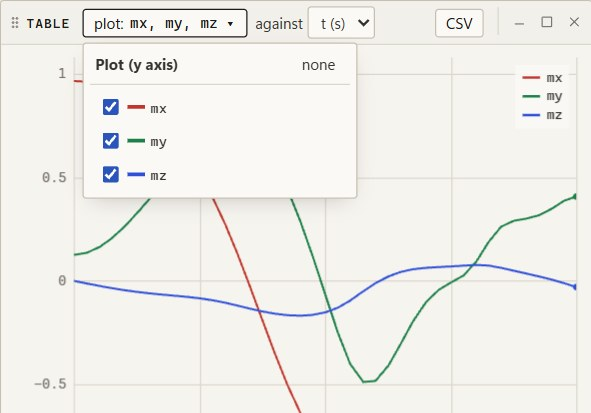
\includegraphics[width=0.6\linewidth]{fig/plot_menu.jpg}
\caption{The table panel with the \menu{plot} menu open: $\langle m_x\rangle$, $\langle m_y\rangle$ and
$\langle m_z\rangle$ of standard problem 4 against time.}
\label{fig:plotmenu}
\end{figure}

\section{The viewer}

There is one viewer, and it works in three dimensions (Figure~\ref{fig:3d}). It draws a vector field as arrows,
cones or cells, coloured like mumax3 (hue from the in-plane angle, lightness from $m_z$), by one component, or by
the magnitude; a scalar quantity is drawn as cells on a diverging scale. Its sources are chosen in the first menu:
\begin{itemize}
\item \menu{Live simulation}: the running or last simulation, refreshed about once a second during a run. The
second menu chooses the quantity: \code{m}, \code{B\_eff}, \code{B\_demag}, \code{B\_exch}, the torques,
\code{SOTorque}, energy densities, the MFM image and others.
\item \menu{Files}: an OVF file, or a series of OVF files with the same prefix, opened with \menu{view} on the
\menu{Files} page; OVF files from anywhere on the computer, opened with \menu{OVF\ldots} or dropped onto the
viewer. Files from outside the output folder are read in the window; they are not copied.
\end{itemize}
OVF 1 and OVF 2 are supported, in text, binary-4 and binary-8 encodings.

\begin{figure}[htbp]
\centering
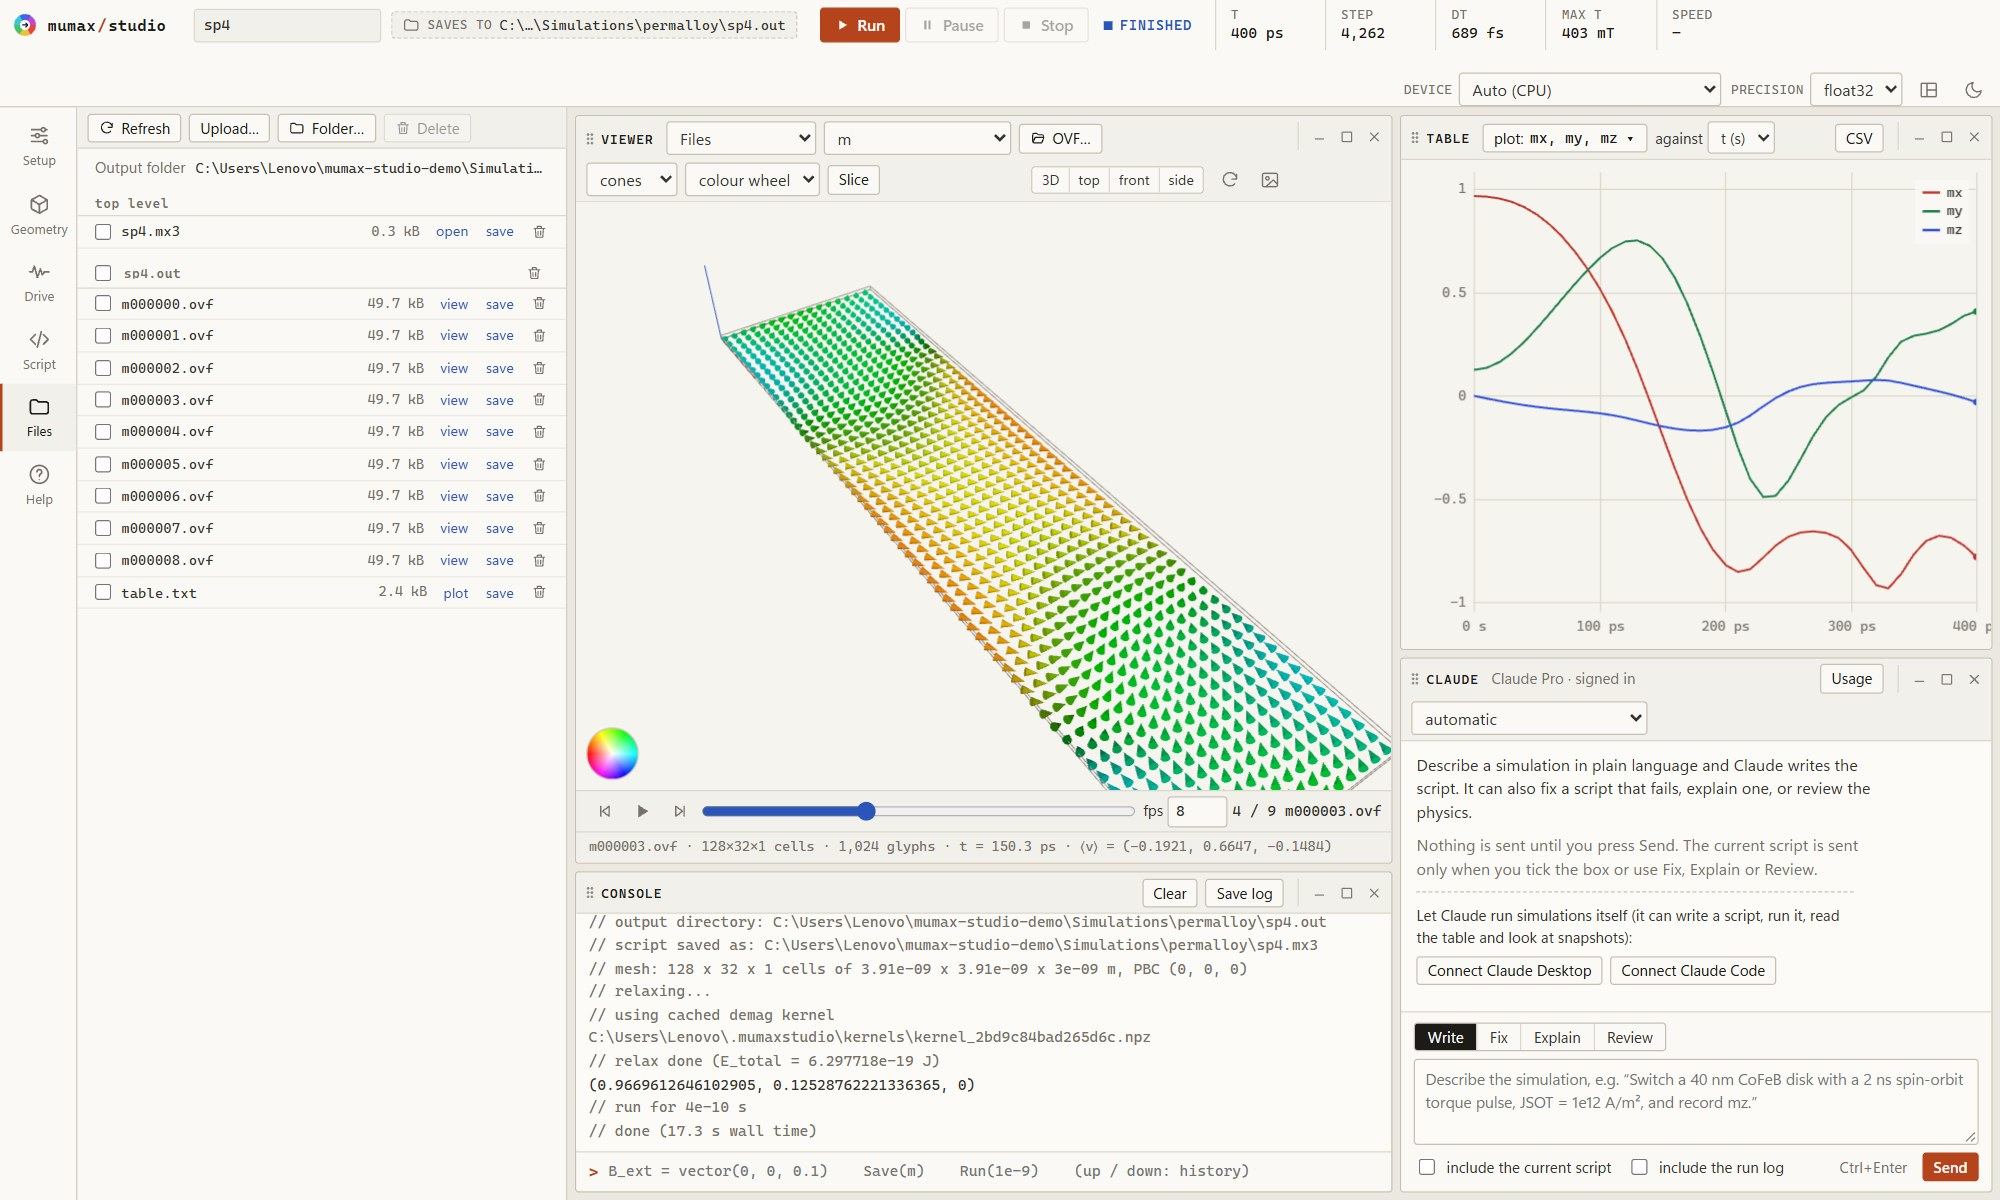
\includegraphics[width=\linewidth]{fig/ui_3d.jpg}
\caption{A series of OVF snapshots of standard problem 4 in the viewer, drawn as cones. \menu{view} on the Files
page loaded the series; the frame bar under the picture steps through it or plays it.}
\label{fig:3d}
\end{figure}

The left mouse button orbits, the right button (or Shift with the left) pans, the wheel zooms. The camera buttons
give the perspective view (\menu{3D}) and the views from \menu{top} ($+z$), \menu{front} ($-y$) and \menu{side}
($+x$); \menu{top} with \menu{cells} reproduces the flat picture of a film. The \menu{Slice} menu restricts the view
to ranges of $x$, $y$ and $z$, which is how the inside of a 3D magnet is seen, and sets the stride (every $n$-th
cell) and the glyph size. With a series loaded, the frame bar steps through the files or plays them at a chosen
rate. The image button saves the picture as PNG. Large meshes are thinned before they are sent to the window; the
info line under the picture says when, and gives the time and the average of the field shown.

While the \menu{Geometry} page is open and nothing runs, the viewer shows the magnet being built instead
(Section~\ref{sec:geomui}); the field shown before comes back when another page is chosen.

\section{Managing files}\label{sec:files}

The \menu{Files} page lists the output folder, three folder levels deep, grouped by folder. The line at the top
gives its full path; \menu{Folder\ldots} changes it (Section~\ref{sec:folder}) and, in the desktop window,
\menu{Open} shows it in the system file manager. Each row offers the actions that fit the file: \menu{view},
\menu{plot}, \menu{open} and \menu{save}.

\paragraph{Deleting.} Files and whole folders can be deleted from the program (Figure~\ref{fig:files}):
\begin{itemize}
\item the bin button at the end of a row deletes that file; on a folder header it deletes the folder and
everything in it;
\item tick several files or folders and press \menu{Delete} in the toolbar to delete them together.
\end{itemize}
A confirmation lists what will be deleted and from which folder. Deleting cannot be undone: the files do not go
to the recycle bin. The result folder of a simulation that is still running is marked \menu{running} and cannot be
deleted, nor can anything in it; stop the run first. The output folder itself is never deleted from here.

\begin{figure}[htbp]
\centering
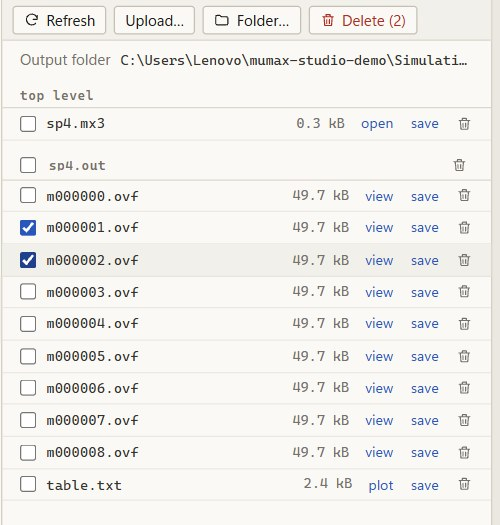
\includegraphics[width=0.62\linewidth]{fig/files_delete.jpg}
\caption{The Files page with two snapshots ticked. \menu{Delete (2)} removes them after a confirmation; the bin
buttons delete single files, or a whole \code{.out} folder from its header.}
\label{fig:files}
\end{figure}

\section{Converting files}

\begin{shell}
$ mumax-studio convert m000010.ovf --png --csv --npy
\end{shell}
writes an image, a CSV table of all cells and a NumPy array of shape $(n_\text{comp}, N_z, N_y, N_x)$.

% =====================================================================
\chapter{Python scripts}\label{ch:python}

\section{Python with the mumax3 names}

A file with the extension \code{.py} runs in the same environment as an \code{.mx3} script, so every mumax3
name exists, and all of Python and NumPy is available:
\begin{pycode}
SetGridSize(64, 64, 1); SetCellSize(4e-9, 4e-9, 4e-9)
Msat = 800e3; Aex = 13e-12; alpha = 0.02
B_ext = lambda t: (5e-3*cos(2*pi*1e9*t), 5e-3*sin(2*pi*1e9*t), 0)
for k in range(3):
    Run(0.5e-9)
    print(t, m.average())
\end{pycode}
Shapes and field terms may be Python functions evaluated on all cells at once:
\begin{pycode}
SetGeom(lambda x, y, z: (x**2 + y**2 < (50e-9)**2) & (abs(z) < 2e-9))

def oersted(x, y, z, t):            # tesla
    B = 1e-3 * Gaussian(t, 0.5e-9, 0.1e-9)
    return (0*x, B*np.tanh(x/20e-9), 0*z)
AddFieldTerm(oersted)
TableAdd(B_custom)
\end{pycode}

\section{The engine as a library}

\begin{pycode}
from mumaxstudio import Simulation, Uniform

sim = Simulation(backend="auto", precision="single")
sim.SetGridSize(128, 32, 1)
sim.SetCellSize(500e-9/128, 125e-9/32, 3e-9)
sim.Msat = 800e3; sim.Aex = 13e-12; sim.alpha = 0.02
sim.m = Uniform(1, .1, 0)
sim.Relax()
print(sim.m_q.Average())
\end{pycode}
\code{backend} is \code{"cpu"}, \code{"gpu"}, \code{"gpu:1"} (a particular card) or \code{"auto"}.

\section{Figures}

\code{matplotlib} is included. In a script run from the interface, \code{plt.show()} saves the current figure as
\code{figure\_001.png}, \code{figure\_002.png}, \ldots{} in the output folder instead of opening a window.

% =====================================================================
\chapter{mumax+ scripts}\label{ch:plus}

\section{The interface}

A Python script that imports \code{mumaxplus} runs against a reimplementation of the mumax+ interface on the
mumax Studio engine. Standard problem 4 in mumax+ form:
\begin{pycode}
from mumaxplus import World, Grid, Ferromagnet

world = World(cellsize=(500e-9/128, 125e-9/32, 3e-9))
magnet = Ferromagnet(world, Grid((128, 32, 1)))
magnet.msat = 800e3
magnet.aex = 13e-12
magnet.alpha = 0.02
magnet.magnetization = (1, 0.1, 0)
magnet.minimize()
print(magnet.magnetization.average())

world.bias_magnetic_field = (-24.6e-3, 4.3e-3, 0)
world.timesolver.run(1e-9)
\end{pycode}
Such a script is run as plain Python: the mumax3 names are not injected, so a variable called \code{m} does not
collide with the magnetization of the mumax3 interpreter.

\section{What is implemented}

\begin{itemize}
\item \code{World}, \code{Grid}, \code{Ferromagnet}, and the two-sublattice \code{Antiferromagnet} and
\code{Ferrimagnet} with \code{sub1}, \code{sub2}, \code{afmex\_cell}, \code{afmex\_nn} and \code{latcon}.
\item Parameters given as numbers, vectors, NumPy arrays, functions of position \code{f(x, y, z)} or of time;
\code{set\_in\_region}, \code{add\_time\_term}.
\item The DMI tensor (\code{set\_interfacial\_dmi}, \code{set\_bulk\_dmi}), \code{inter\_exchange} and
\code{scale\_exchange} between regions.
\item Rigid magneto-elastic strain (\code{B1}, \code{B2}, \code{rigid\_norm\_strain},
\code{rigid\_shear\_strain}); Zhang--Li and Slonczewski torques; temperature.
\item \code{world.timesolver} with \code{run}, \code{steps}, \code{run\_while}, \code{solve}, \code{time},
\code{timestep}, \code{adaptive\_timestep}, \code{max\_error}, \code{headroom} and \code{set\_method};
\code{relax} and \code{minimize}.
\item Field and energy quantities, including the energy densities of each term; \code{.eval()} returns a NumPy
array of shape $(n_\text{comp}, N_z, N_y, N_x)$ and \code{.average()} a tuple.
\item The \code{mumaxplus.util} helpers: shapes, \code{VoronoiTessellator}, \code{neelskyrmion},
\code{vortex}, \code{twodomain}, \code{plot\_field}, \code{show\_layer} and \code{show\_regions}.
\end{itemize}

\section{Verification}

The following examples from the mumax+ repository were run unchanged and gave the physically expected results:
standard problem 4, anisotropy, the LL torque example, MRAM bit switching, the skyrmion racetrack, Voronoi
grains, antiferromagnetic resonance, periodic boundary conditions and the multilayer example. The comparison is
qualitative where the mumax+ repository publishes figures rather than numbers. The sign convention of the DMI of
mumax+ could not be compared with mumax+ itself, which needs an NVIDIA GPU; it follows the mumax+ documentation.

\section{What is missing}

Non-collinear antiferromagnets (\code{NcAfm}), altermagnets, elastodynamics (time-resolved strain), the Poisson
current solver, moving windows and the inter-sublattice DMI are not implemented. A world holds either
ferromagnets or a single antiferromagnet or ferrimagnet. Ferromagnets in the same world interact only through their
stray fields, as in mumax+.

% =====================================================================
\chapter{Worked examples}\label{ch:examples}

Each example in this chapter is a complete simulation that ships with the program: on the \menu{Script} page,
choose it from \menu{Examples}, set a name, and press \menu{Run}. For each one the chapter says how the same
simulation is put together with the forms, what to look at while it runs, and what it gave on the computer on
which this book was written (a laptop processor, single precision; times are wall-clock times). Your numbers
may differ in the last digits.

\section{A skyrmion in a nanodisk}

\paragraph{Goal.} Stabilise a N\'eel skyrmion in a Co/Pt-like disk with perpendicular anisotropy and interfacial
DMI, then make it breathe with an oscillating perpendicular field. Example \menu{02 skyrmion dmi}.

\paragraph{With the forms.}
\begin{enumerate}
\item \menu{Geometry}: mesh $64\times64\times1$, cells $2\times2\times0.6$\,nm$^3$; add a \menu{Disk} of
120\,nm.
\item \menu{Setup}: preset \menu{Co/Pt with DMI (skyrmions)} ($M_s = 580$\,kA/m, $A = 15$\,pJ/m,
$K_{u1} = 0.8$\,MJ/m$^3$, $D_\text{ind} = 3$\,mJ/m$^2$, $\alpha = 0.3$); initial state \menu{N\'eel skyrmion},
charge 1, polarity $-1$; keep \menu{Relax first}; tick \menu{topological charge} in the table columns.
\item \menu{Drive}: under \menu{External field} add a term along $z$ with amplitude 20\,mT and the waveform
\menu{Sine (continuous wave)} at 2\,GHz.
\end{enumerate}

\paragraph{The script.}
\begin{mxcode}
SetGridSize(64, 64, 1)
SetCellSize(2e-9, 2e-9, 0.6e-9)
SetGeom(Circle(120e-9))
Msat = 580e3;  Aex = 15e-12;  Ku1 = 0.8e6;  anisU = vector(0, 0, 1)
Dind = 3.0e-3; alpha = 0.3
m = NeelSkyrmion(1, -1)          // core down, background up
Relax()
print("skyrmion number Q =", ext_topologicalcharge.get())
Save(m)
alpha = 0.05
B_ext = vector(0, 0, 0.02 * sin(2*pi*2e9*t))
TableAdd(ext_topologicalcharge)
TableAdd(B_ext)
TableAutoSave(10e-12)
Run(1e-9)
\end{mxcode}

\paragraph{What to look at.} In the viewer, choose \menu{top} and \menu{cells}: the core is black (down) in a
white (up) disk, ringed by the colours of the in-plane wall. In the table panel, choose \code{mz} and
\code{ext\_topologicalcharge} in the \menu{plot} menu: $\langle m_z\rangle$ oscillates at 2\,GHz as the skyrmion grows and shrinks.

\paragraph{Result.} After the relaxation $Q = -0.854$ and $\langle m_z\rangle = 0.953$; $Q$ stays at
$-0.854$ during the field cycle, so the skyrmion survives. $|Q|$ is below 1 because the DMI tilts the
magnetization at the edge of the disk, which contributes to the integral with the opposite sign. The run takes
about 85\,s.

\section{Vortex gyration and its frequency}

\paragraph{Goal.} Find the frequency of the gyrotropic mode of a vortex in a permalloy disk of 256\,nm diameter
and 20\,nm thickness, by exciting it with a field pulse and Fourier-transforming the response. Example
\menu{10 vortex frequency} (Python).

\paragraph{The script.}
\begin{pycode}
import numpy as np
import matplotlib.pyplot as plt

SetGridSize(64, 64, 1)
SetCellSize(4e-9, 4e-9, 20e-9)
SetGeom(Circle(256e-9))
Msat = 860e3; Aex = 13e-12; alpha = 0.01
m = Vortex(1, 1)
Relax()

B_ext = vector(5e-3, 0, 0)        # 5 mT for 100 ps pushes the core aside
Run(100e-12)
B_ext = vector(0, 0, 0)

interval = 10e-12                 # (dt and step are built-in names)
ts, mx = [], []
for i in range(500):              # 5 ns of free gyration
    Run(interval)
    ts.append(i * interval)
    mx.append(m.average()[0])
# ... FFT of <mx>(t), zero crossings, and a plot (see the example file)
plt.show()
\end{pycode}
The loop is the Python way of recording a signal: instead of a table, the values are collected in a list and
analysed with NumPy in the same script. The full example estimates the frequency twice, from the peak of the FFT
and from the time between upward zero crossings, which is more precise when only a few periods are recorded.

\paragraph{Result.} The script prints
\begin{shell}
gyration frequency: 678 MHz from 3 periods (FFT peak 662 MHz)
\end{shell}
and saves Figure~\ref{fig:exvortex} as \code{figure\_001.png} in the result folder. A 5\,ns record resolves
the frequency only to about $1/5\,\text{ns} = 200$\,MHz in the FFT; run longer (more loop passes) for a sharper
peak. The core also rings at higher frequencies just after the pulse, visible as the fast wiggles of the first
nanosecond. The run takes about 40\,s.

\begin{figure}[htbp]
\centering
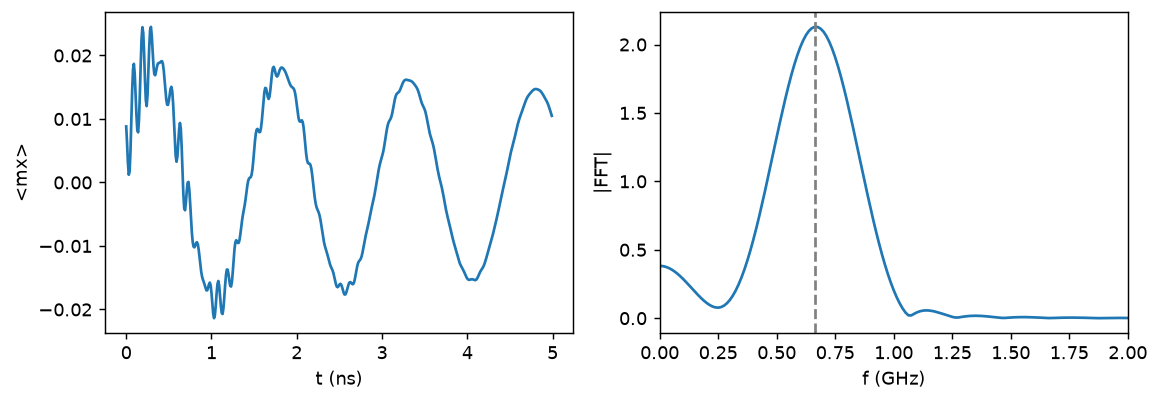
\includegraphics[width=0.95\linewidth]{fig/ex_vortex.png}
\caption{Output of \menu{10 vortex frequency}: $\langle m_x\rangle(t)$ after the pulse (left) and its spectrum
(right), with the peak near 0.66\,GHz.}
\label{fig:exvortex}
\end{figure}

\section{A hysteresis loop in Python}

\paragraph{Goal.} The hysteresis loop of a $128\times128\times4$\,nm$^3$ permalloy square, with the field
steps made by NumPy and the loop drawn by matplotlib. Example \menu{11 hysteresis python}; the \code{.mx3}
version with Go-style loops is \menu{07 hysteresis loop}.

\paragraph{The script.}
\begin{pycode}
import numpy as np
import matplotlib.pyplot as plt

SetGridSize(32, 32, 1)
SetCellSize(4e-9, 4e-9, 4e-9)
Msat = 800e3; Aex = 13e-12; alpha = 0.5
m = Uniform(1, 0.01, 0)

down = np.linspace(60e-3, -60e-3, 61)            # 2 mT steps
fields = np.concatenate([down, down[::-1]])
mx = []
for b in fields:
    B_ext = vector(b, 1e-3, 0)    # a small y field breaks the symmetry
    Minimize()
    mx.append(m.average()[0])
    TableSave()
# coercive field and plot: see the example file
\end{pycode}
\code{Minimize} finds the equilibrium at each field without following the dynamics, which is what a
quasi-static loop needs and much faster than \code{Run}. \code{TableSave} adds one row per field, so the loop
can also be plotted in the table panel: choose \menu{plot: mx} \menu{against B\_extx} (add
\code{TableAdd(B\_ext)} to the script for the field column).

\paragraph{Result.} The square switches between $-6$ and $-8$\,mT on the way down (the script prints
\code{coercive field (down branch): 8 mT}, the first step at which $\langle m_x\rangle < 0$) and symmetrically
on the way up (Figure~\ref{fig:exhyst}). Before switching, $\langle m_x\rangle$ falls gradually as the
magnetization at the edges turns. 122 minimisations take about 35\,s.

\begin{figure}[htbp]
\centering
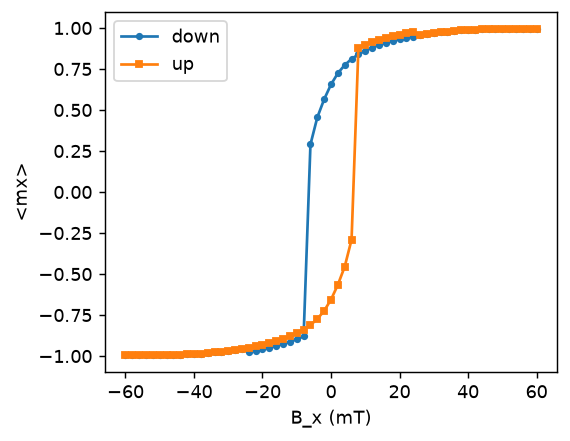
\includegraphics[width=0.55\linewidth]{fig/ex_hysteresis.png}
\caption{The loop drawn by \menu{11 hysteresis python}.}
\label{fig:exhyst}
\end{figure}

\section{A domain wall pushed by a current}

\paragraph{Goal.} Move a domain wall in a perpendicular nanostrip with a spin-polarised current (Zhang--Li
torque) and measure its speed. Example \menu{06 domain wall current}.

\paragraph{With the forms.} \menu{Geometry}: mesh $256\times32\times1$ of $2\times2\times1$\,nm$^3$, no shapes.
\menu{Setup}: preset \menu{CoFeB, perpendicular}, then set $M_s = 600$\,kA/m, $A = 10$\,pJ/m,
$K_{u1} = 0.6$\,MJ/m$^3$, $\alpha = 0.02$; initial state \menu{Two domains, up | down}; tick \menu{DW position}.
\menu{Drive}: under \menu{Spin-transfer current} add a term along $x$ of 100\,MA/cm$^2$
($10^{12}$\,A/m$^2$) with the waveform \menu{Constant (DC)}, and set polarization 1 and non-adiabaticity
$\xi = 0.04$. (The form's two-domain state has a N\'eel wall; the example script starts from a Bloch wall.)

\paragraph{The script.}
\begin{mxcode}
SetGridSize(256, 32, 1)
SetCellSize(2e-9, 2e-9, 1e-9)
Msat = 600e3; Aex = 10e-12; Ku1 = 0.6e6; anisU = vector(0, 0, 1)
alpha = 0.02; xi = 0.04; Pol = 1
m = TwoDomain(0, 0, 1,  1, 1, 0,  0, 0, -1)   // up | Bloch wall | down
Relax()
J = vector(1e12, 0, 0)
TableAdd(ext_dwpos)
TableAutoSave(10e-12)
AutoSave(m, 200e-12)
Run(1e-9)
print("wall position:", ext_dwpos.get(), "m")
\end{mxcode}

\paragraph{Result.} The wall moves against the current, along the electron flow: \code{ext\_dwpos} is
$-47$\,nm at 0.5\,ns and $-96$\,nm at 1\,ns, a steady 96\,m/s. This is close to the spin-drift velocity
$u = \mu_B P J/(eM_s) = 97$\,m/s. The in-plane angle of the wall turns slowly during the run (from $90^\circ$ to
about $68^\circ$, read from $\langle m_x\rangle$ and $\langle m_y\rangle$), so the wall is not in the
rigid steady state of the one-dimensional model, which would give $v = (\xi/\alpha)u$. Use the OVF snapshots
and the viewer's frame bar to watch the wall travel. The run takes about 3 minutes.

\section{Spin-orbit torque switching}

Chapter~\ref{ch:torques} works through the switching of a perpendicular disk by a spin-orbit torque pulse;
the same simulation is example \menu{03 sot switching}. As an exercise, change the sign of \code{JSOT} and the
amplitude of the pulse, and find the current below which the magnet no longer switches.

\section{A geometry made in Python}

\paragraph{Goal.} Combine the Python geometry methods of Section~\ref{sec:geompy} in one script and look at how
holes bend the magnetization. Example \menu{12 geometry python}.

\begin{pycode}
import numpy as np
SetGridSize(192, 96, 1)
SetCellSize(4e-9, 4e-9, 4e-9)

film = Rect(768e-9, 384e-9)                      # 1. antidot lattice made in a loop
for ix in range(-3, 4):
    for iy in range(-1, 2):
        film = film.Sub(Circle(50e-9).Transl(ix * 110e-9, iy * 110e-9, 0))

rng = np.random.default_rng(3)                   # 2. random defects, reproducible
for cx, cy in rng.uniform([-360e-9, -170e-9], [360e-9, 170e-9], size=(8, 2)):
    film = film.Sub(Circle(12e-9).Transl(cx, cy, 0))
SetGeom(film)

DefRegion(1, lambda x, y, z: x > 0)              # 3. region from a function

Msat = 800e3; Aex = 13e-12; alpha = 0.5
Msat.SetRegion(1, 600e3)                         # a softer right half
m = Uniform(1, 0.1, 0)
B_ext = vector(20e-3, 0, 0)
Minimize()
print("<m> =", m.average())
Save(m)
Save(regions)
\end{pycode}

\paragraph{Result.} The log reports \code{// geometry: 15812 / 18432 cells}; the minimisation ends at
$\langle\mathbf m\rangle = (0.966, 0.091, 0)$ after about 5\,s. Open \code{m000000.ovf} with \menu{view} on the
Files page and \code{regions000000.ovf} beside it: the magnetization bends around every hole, most strongly at
the free ends of the film (Figure~\ref{fig:exantidot}).

\begin{figure}[htbp]
\centering
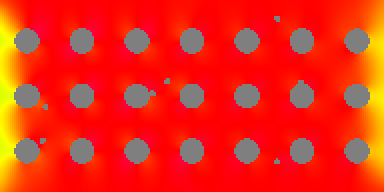
\includegraphics[width=0.6\linewidth]{fig/ex_antidots.png}
\caption{The minimised state of \menu{12 geometry python}, converted with
\code{mumax-studio convert m000000.ovf --png}. Holes and defects are grey.}
\label{fig:exantidot}
\end{figure}

\section{From an example to your own study}

The examples are starting points. A typical way to turn one into a study is:
\begin{enumerate}
\item load the example, give the simulation a name of its own, and check the output folder in the top bar;
\item make the run short (a smaller mesh, a shorter \code{Run}) and check the geometry, the initial state and
the first table rows;
\item restore the full size and run; keep the script with \menu{Save\ldots} next to your notes;
\item for a parameter sweep, put the run in a loop (Chapter~\ref{ch:advanced}), or save one script per value
and run them with \code{mumax-studio run};
\item delete result folders you no longer need from the Files page.
\end{enumerate}


% =====================================================================
\chapter{Devices and performance}\label{ch:perf}

\section{The benchmark}

\code{mumax-studio bench} measures the wall time of one solver step for a range of mesh sizes on every engine it
finds: the processor in single and double precision, the processor with a single FFT thread, and each GPU in both
precisions. The test problem is a permalloy film of $N\times N\times1$ cells of $2\times2\times2$\,nm$^3$ with
exchange, demagnetisation and a static field, in a vortex state, integrated with the Dormand--Prince method at a
fixed step. A 3D mesh of $128\times128\times16$ cells is added. The first steps, which include building the demag
kernel and compiling GPU kernels, are not timed.
\begin{shell}
$ mumax-studio bench                       # all engines, CSV and PNG
$ mumax-studio bench --engines cpu,gpu:0 --sizes 64,256,1024
\end{shell}

\section{Measured results}

Figure~\ref{fig:bench} and Table~\ref{tab:bench} show the results on the computer on which this book was
written: an AMD Ryzen 5 7520U with Radeon Graphics with 8 threads, Windows 11, Python 3.11.5, mumax Studio 0.3.0\unskip.

\begin{figure}[htbp]
\centering
\IfFileExists{bench_cpu.pdf}{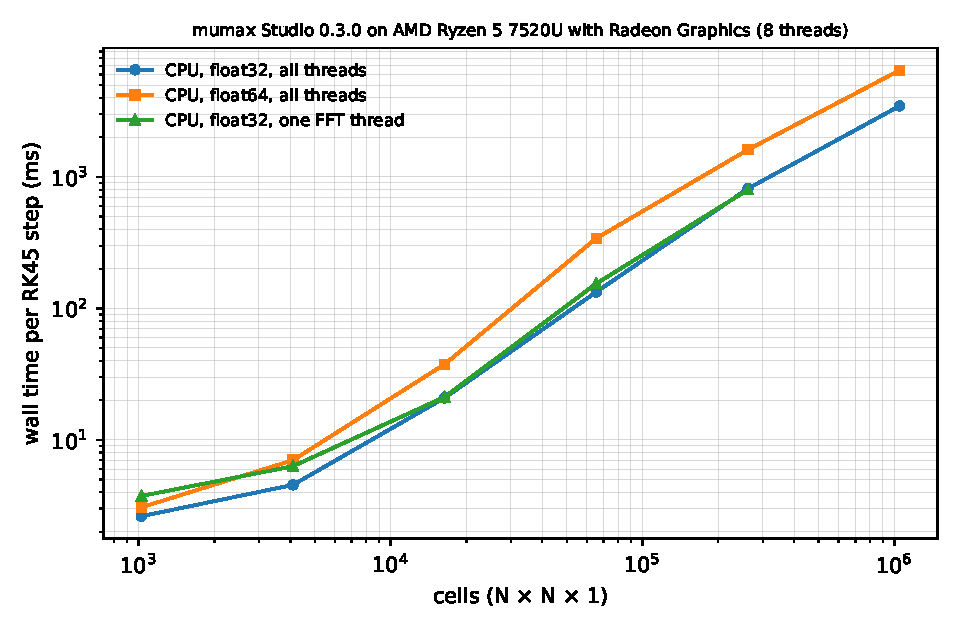
\includegraphics[width=0.92\linewidth]{bench_cpu.pdf}}{\fbox{benchmark figure}}
\caption{Wall time per Dormand--Prince step against the number of cells for an $N\times N\times1$ permalloy film.
Measured with \code{mumax-studio bench}.}
\label{fig:bench}
\end{figure}

\begin{table}[htbp]
\centering
\caption{Time per step (ms) and throughput (million cells per second).}
\label{tab:bench}
\begin{tabular}{l rr rr rr}
\toprule
 & \multicolumn{2}{c}{CPU float32} & \multicolumn{2}{c}{CPU float64} & \multicolumn{2}{c}{float32, 1 FFT thread}\\
\cmidrule(lr){2-3}\cmidrule(lr){4-5}\cmidrule(lr){6-7}
Mesh & ms & Mcell/s & ms & Mcell/s & ms & Mcell/s\\
\midrule
$32\times32\times1$ & 2.6 & 0.39 & 3.1 & 0.33 & 3.7 & 0.27\\
$64\times64\times1$ & 4.5 & 0.90 & 7.0 & 0.59 & 6.3 & 0.65\\
$128\times128\times1$ & 20.9 & 0.79 & 37.6 & 0.44 & 21.2 & 0.77\\
$256\times256\times1$ & 133 & 0.49 & 341 & 0.19 & 154 & 0.42\\
$512\times512\times1$ & 815 & 0.32 & 1609 & 0.16 & 798 & 0.33\\
$1024\times1024\times1$ & 3465 & 0.30 & 6470 & 0.16 & -- & --\\
$128\times128\times16$ & 1518 & 0.17 & 2773 & 0.09 & 1510 & 0.17\\
\bottomrule
\end{tabular}

\end{table}

\paragraph{GPU results.} The computer on which this book was written has no NVIDIA graphics card, so no GPU
figures are given; numbers that were not measured are not reported. To add them, run \code{mumax-studio bench}
on a machine with an NVIDIA card: the GPU curves are drawn in the same figure, and the CSV files of several
machines can be combined and redrawn with \code{mumaxstudio.bench.plot\_csv}.

\section{Reading the results}

The step time grows slightly faster than linearly with the number of cells, as the FFT of the demagnetising
convolution has cost $O(N\log N)$ on a grid padded to twice its size. On the processor, double precision costs
about a factor of two. The curve for a single FFT thread lies almost on the curve for all eight threads: on the
processor the FFT is not the bottleneck. The element-wise NumPy operations of the field terms and the solver are,
and NumPy runs them on one core. Throughput is highest near $10^4$ cells, where the arrays still fit in the
processor cache. A practical rule follows: on a laptop processor, meshes up to about $10^5$ cells give
interactive speed; beyond that a GPU, or mumax3 itself, is the better tool.

% =====================================================================
\chapter{Working with Claude}\label{ch:claude}

mumax Studio can ask Claude to write, correct, explain or review scripts, and Claude Desktop or Claude Code can
run simulations through mumax Studio themselves. None of this is needed to use the program, and nothing is sent
anywhere until you press \menu{Send}.

\section{Authorizing Claude with a Pro or Max account}

The Claude panel is locked until it is authorized: it shows the steps below instead of the request box. It is
authorized by signing in with a \emph{Claude Pro or Max} account (a Team or Enterprise seat also works); a free
Claude account is not enough. mumax Studio reaches Claude through Claude Code, Anthropic's command-line program,
which keeps the sign-in.
\begin{enumerate}
\item \textbf{Install Claude Code.} On Windows, in PowerShell: \code{irm https://claude.ai/install.ps1 | iex};
on macOS and Linux: \code{curl -fsSL https://claude.ai/install.sh | bash}; or see
\url{https://claude.com/claude-code}. Press \menu{Check again}; the first step is ticked.
\item \textbf{Sign in.} Press \menu{Sign in with Claude}. A terminal window opens with \code{claude auth login},
and the browser shows the Claude sign-in page. Sign in with your Pro or Max account and allow the access. The
panel checks every few seconds and unlocks by itself; the status line then reads
\menu{Claude Pro \textperiodcentered{} signed in}.
\end{enumerate}
If Claude Code is signed in with an account without a subscription, the panel says so and offers
\menu{Sign out of this account} and \menu{Sign in with another account}. Requests count towards the usage limits
of your plan; no API key is involved and nothing is billed separately.

\paragraph{Watching the usage.} Once Claude is authorized, the \menu{Usage} button in the panel's title bar shows
how much of the plan's limits is used, as in Claude itself: the current session (a five-hour window) and the
week, each as a percentage with a bar and the time at which it resets. The figures come with every answer from
Claude, so they are up to date after each request; \menu{Refresh} fetches them at once (with a one-word request to
the smallest model, which itself counts a negligible amount). The bar turns amber above 80\,\% and red when a limit
is reached. The same box names the signed-in account and has \menu{Sign out} (Figure~\ref{fig:usage}).

\begin{figure}[htbp]
\centering
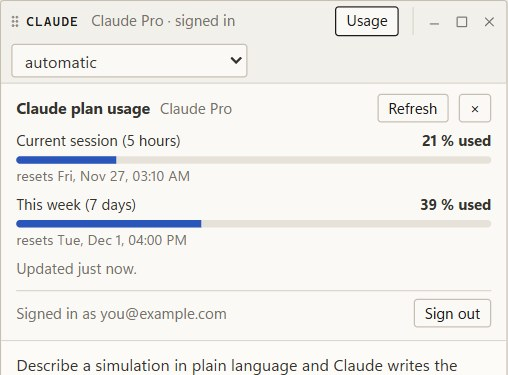
\includegraphics[width=0.6\linewidth]{fig/claude_usage.jpg}
\caption{\menu{Usage} in the Claude panel: the share of the plan's five-hour and weekly limits used so far, and
when each resets.}
\label{fig:usage}
\end{figure}

\section{Connecting with an API key}

Without a subscription, an Anthropic API key can be used instead (\menu{Use an API key instead} in the locked
panel). Create one at \url{https://console.anthropic.com}, paste
it into the key field of the Claude panel and press \menu{Save}. The key is stored in
\code{\textasciitilde/.mumaxstudio/config.json}, readable only by your user account; the environment variable
\code{ANTHROPIC\_API\_KEY} is used instead if it is set. A pip installation needs \code{pip install anthropic}
for this route. Usage is billed to the API account.

\begin{figure}[htbp]
\centering
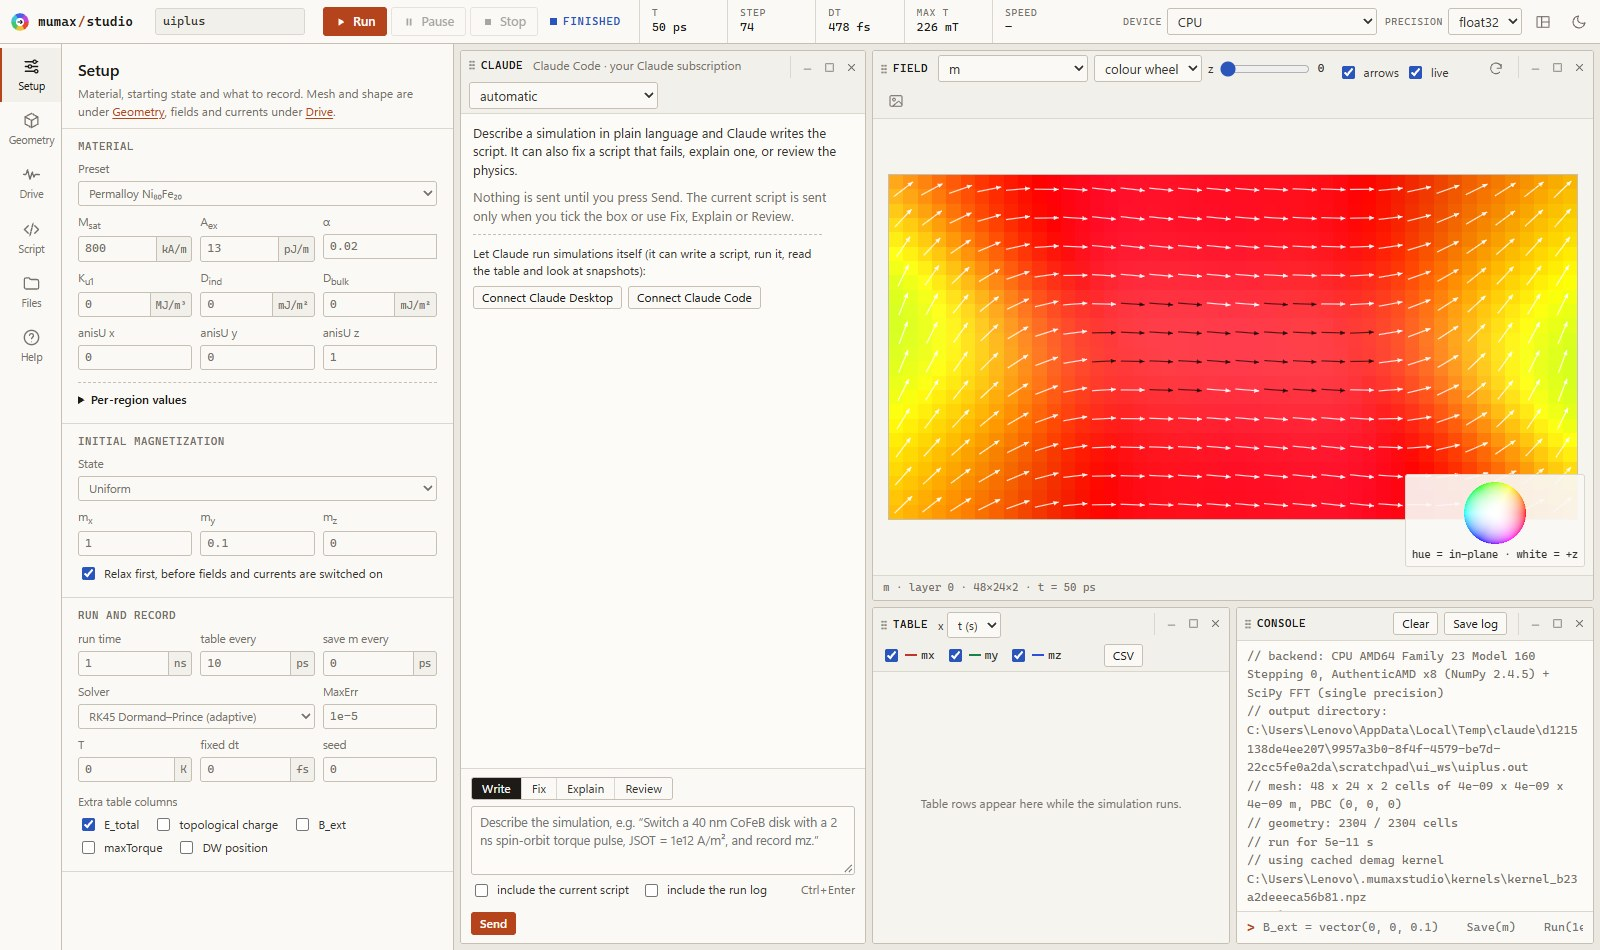
\includegraphics[width=\linewidth]{fig/ui_claude.jpg}
\caption{The \menu{Writing with Claude} arrangement: the Claude panel, connected through Claude Code, beside
the viewer, the plot and the console.}
\label{fig:claude}
\end{figure}

\section{Asking for a script}

The panel has four modes:
\begin{description}
\item[Write] describes a simulation in words and receives a script. Tick \menu{include the current script} to
have it extended rather than written from scratch.
\item[Fix] sends the current script and its last error message and receives a corrected script.
\item[Explain] receives an explanation of the physics and of each block of the current script.
\item[Review] receives a check of cell size, time step, units and boundary conditions.
\end{description}
An answer that contains a script has the buttons \menu{Put in editor}, \menu{Put in editor and run} and
\menu{Copy}. A good request names the material, the geometry with its dimensions, the excitation and what is to be
recorded, for example:
\begin{quote}\itshape
Switch a 40 nm CoFeB disk, 1 nm thick, with perpendicular anisotropy, using a 2 ns spin-orbit torque pulse of
$1.2\times10^{12}$ A/m$^2$ from a tungsten layer, with a 20 mT in-plane field along $x$; record $m_z$ every 10 ps.
\end{quote}
Read a generated script before trusting its results. Claude is generally reliable with the syntax but can choose
parameters that are physically doubtful; the \menu{Review} mode and Chapter~\ref{ch:mx3} help to check them.

\section{Letting Claude run simulations (MCP)}

mumax Studio contains a Model Context Protocol server. A client that speaks MCP, such as Claude Desktop or Claude
Code, can then call these tools:
\begin{center}
\begin{tabular}{>{\raggedright\ttfamily}p{0.3\linewidth} p{0.62\linewidth}}
\toprule
run\_simulation & run an \code{.mx3}, Python or mumax+ script and return the log, the final averages and the
last table rows \\
describe\_api & the script languages, for reference \\
list\_examples, read\_example & the bundled examples \\
list\_outputs, read\_table & files of earlier runs, and their tables \\
render\_ovf & an OVF snapshot as an image that Claude can look at \\
system\_info & version, devices and output folder \\
\bottomrule
\end{tabular}
\end{center}
In the Claude panel, \menu{Connect Claude Desktop} adds the server to Claude Desktop's configuration (keeping
other entries and a backup of the file); restart Claude Desktop afterwards. \menu{Connect Claude Code} registers it
for your user with Claude Code. By hand, the equivalent is
\begin{shell}
$ claude mcp add --scope user mumax-studio -- mumax-studio mcp
\end{shell}
or, in \code{claude\_desktop\_config.json},
\begin{lstlisting}
{ "mcpServers": { "mumax-studio": { "command": "mumax-studio", "args": ["mcp"] } } }
\end{lstlisting}
with the full path of \code{mumax-studio.exe} on Windows if it is not on the \code{PATH}. A conversation can then
proceed as: ``Find the field at which a $200\times50\times5$\,nm$^3$ permalloy bar switches along its long axis,
and show me the state just before switching.'' Claude writes the script, runs it, reads the table and inspects the
snapshots. Simulations started this way run in the output folder last chosen in mumax Studio
(\code{\textasciitilde/mumax-studio} if none was chosen), or in the folder given by the environment variable
\code{MUMAXSTUDIO\_WORKSPACE} or the option \code{--workspace}, and appear on the \menu{Files} page.

% =====================================================================
\chapter{Advanced use}\label{ch:advanced}

\section{Parameter sweeps}

A sweep is a loop in the script. The following finds the switching field of a bar by stepping the field and
minimising at each step; every step adds one table row:
\begin{mxcode}
SetGridSize(100, 25, 1); SetCellSize(2e-9, 2e-9, 5e-9)
Msat = 800e3; Aex = 13e-12; alpha = 1
m = Uniform(1, 0, 0)
TableAdd(B_ext)
for B := 0.0; B >= -0.1; B -= 0.002 {
    B_ext = vector(B, 1e-4, 0)
    Minimize()
    TableSave()
}
\end{mxcode}
For sweeps that should run in parallel, write one script per value and start them with
\code{mumax-studio run a.mx3 b.mx3 ...}.

\section{Custom field terms}

Besides Python functions, mumax3-style quantity arithmetic defines new field terms without Python:
\begin{mxcode}
AddFieldTerm(Mul(Const(0.1), m))        // also Add, Madd, Dot, Cross, MulMV, Masked
\end{mxcode}

\section{Headless runs and remote GPUs}

\code{mumax-studio run sim.mx3 --backend gpu --precision double} runs without an interface and writes
\code{sim.out/} as mumax3 does. To use a GPU server from a laptop, start the interface on the server with
\code{mumax-studio gui --host 0.0.0.0 --port 35367} and open the printed address, including its token, in the
laptop's browser. The token grants the right to run code on the server: keep it private, and prefer an SSH tunnel
(\code{ssh -L 35367:localhost:35367 server}) to exposing the port.

\section{Thermal fluctuations}

\code{Temp} adds the stochastic thermal field. Use a fixed time step, \code{FixDt}, for thermal runs;
\code{ThermSeed} makes them repeatable. Compare averages over several seeds, not single trajectories.

% =====================================================================
\chapter{Validation and known problems}\label{ch:limits}

\section{How the engine is tested}

The test suite (\code{python -m unittest discover -s tests}) checks the engine against analytical results: the
Newell demagnetisation tensor, the demagnetising factors of a cube and of a thin film, the exchange and DMI
fields of spin spirals, Larmor precession, the anisotropy field, and the SOT and Slonczewski torques against the
formulas of the CUDA kernels. It also tests the script language, the OVF format, the mumax+ interface, the
interface server, the MCP server and the benchmark. The fifteen examples of the mumax3 website and nine examples
of the mumax+ repository run to completion with plausible results.

\section{Known problems}

\begin{enumerate}
\item \textbf{The GPU path has not been run on an NVIDIA card} by the author. It uses the same code as the CPU
path through CuPy and passes the self-test logic, but its speed and its numerical agreement with the CPU path are
unverified.
\item \textbf{Speed.} On a processor the program is one to two orders of magnitude slower than mumax3 on a GPU
(Chapter~\ref{ch:perf}), and it uses essentially one core: the multi-threaded FFT makes almost no difference,
because single-threaded element-wise NumPy operations dominate.
\item \textbf{Incomplete mumax3 coverage.} Seventeen of the 295 names of mumax3 3.12 are missing:
\code{GrainRoughness}, \code{Line}, \code{Line2D}, \code{VoxelShape}, \code{HopfionCompactSupport},
\code{ext\_centerWallInLayer}, \code{ext\_centerWallInRegion}, \code{ext\_AllRegionShapes},
\code{ext\_geomEdge}, \code{ext\_grainboundaries}, \code{ext\_grainCutShape}, the Hopf-index and emergent-field
quantities, and \code{ext\_enableCenterBubbleX/Y}. The backward-Euler solver is replaced by Heun's method with a
fixed step.
\item \textbf{Incomplete mumax+ coverage}, as listed in Chapter~\ref{ch:plus}; the DMI sign convention has not
been compared with mumax+ directly.
\item \textbf{Spin-orbit torque uses only the $z$ component of \code{JSOT}}, as the original fork does; a current
in another direction must be expressed through \code{SOTFixedLayer}.
\item \textbf{Defects of the original Go/CUDA fork.} With \code{SOThickness} left at its default of zero, the
CUDA kernel divides by zero and produces NaN; mumax Studio substitutes the mesh thickness. \code{AddSOTorque} in the
Go code reads the spin-transfer current \code{J} instead of \code{JSOT} (the value is not used). Neither is fixed in
the Go code in this repository.
\item \textbf{Magneto-elastic coupling is rigid}: strains are prescribed, not computed.
\item \textbf{Releases are not code-signed}, so Windows and browsers warn about new downloads until the files
gain reputation or are signed.
\item \textbf{The Claude assistant can produce wrong scripts.} Its output must be checked.
\end{enumerate}

\appendix
% =====================================================================
\chapter{Command reference}

\begin{center}
\begin{tabular}{>{\ttfamily}p{0.43\linewidth} p{0.5\linewidth}}
\toprule
mumax-studio & the interface in its own window \\
mumax-studio gui [file] [--port P] [--workspace DIR] [--host H] [--native] & the interface, with options;
\code{--workspace} overrides the remembered output folder \\
mumax-studio run a.mx3 [--backend cpu|gpu|gpu:N] [--precision single|double] & headless run \\
mumax-studio info & version and devices \\
mumax-studio convert f.ovf [--png] [--csv] [--npy] & convert output files \\
mumax-studio bench [--engines ...] [--sizes ...] [--steps n] [--out name] & benchmark \\
mumax-studio mcp [--workspace DIR] & MCP server on standard input and output \\
\bottomrule
\end{tabular}
\end{center}

\chapter{Troubleshooting}

\begin{description}
\item[The GPU is listed but disabled.] Read the reason next to it. ``NVRTC'' or ``cuFFT'' means the CUDA
libraries are missing: use the NVIDIA package, or \code{pip install "cupy-cuda12x[ctk]"}. ``driver'' means the
NVIDIA driver is too old.
\item[The window stays blank.] On Windows the window needs the Edge WebView2 runtime, which Windows 10 and 11
normally include. On Linux it needs the GTK WebKit libraries. The program falls back to the browser; the address
is written to \code{\textasciitilde/mumax-studio/studio.log}.
\item[A download button does nothing.] Inside the desktop window, downloads open a save dialog; if none appears,
check that the dialog has not opened behind the main window.
\item[Run does nothing but open a folder dialog.] No output folder has been chosen yet. Choose one and press
\menu{Use this folder}; the run starts. This happens once.
\item[The Claude panel is locked.] Claude Code is missing, not signed in, or signed in without a Pro or Max plan.
The panel lists what is missing; follow its steps.
\item[The results are not where I expected.] The \menu{saves to} chip in the top bar and the first lines of
the run log give the full path. The output folder is remembered between sessions; change it with the chip.
\item[A file cannot be deleted.] Files of a running simulation are protected: stop it first. On Windows a file
that another program has open (an editor, a plotting program) cannot be deleted until that program closes it;
the console names the file and the reason.
\item[Claude Code is not found.] Make sure \code{claude} runs in a new terminal, then press \menu{Check again}.
\item[A run is slow.] Reduce the mesh, use single precision, use \code{Minimize} rather than \code{Relax} for
static states, and check that the chosen device is the one intended.
\end{description}

\end{document}
